\documentclass[10pt]{article}
\usepackage{NotesTeXV3,lipsum, tikzit}
\usepackage{tikz}
\usetikzlibrary{backgrounds}
\usetikzlibrary{arrows}
\usetikzlibrary{shapes,shapes.geometric,shapes.misc}

% this style is applied by default to any tikzpicture included via \tikzfig
\tikzstyle{tikzfig}=[baseline=-0.25em,scale=0.5]

% these are dummy properties used by TikZiT, but ignored by LaTex
\pgfkeys{/tikz/tikzit fill/.initial=0}
\pgfkeys{/tikz/tikzit draw/.initial=0}
\pgfkeys{/tikz/tikzit shape/.initial=0}
\pgfkeys{/tikz/tikzit category/.initial=0}

% standard layers used in .tikz files
\pgfdeclarelayer{edgelayer}
\pgfdeclarelayer{nodelayer}
\pgfsetlayers{background,edgelayer,nodelayer,main}

% style for blank nodes
\tikzstyle{none}=[inner sep=0mm]

% include a .tikz file
\newcommand{\tikzfig}[1]{%
{\tikzstyle{every picture}=[tikzfig]
\IfFileExists{#1.tikz}
  {\input{#1.tikz}}
  {%
    \IfFileExists{./tikz/#1.tikz}
      {\input{./tikz/#1.tikz}}
      {\tikz[baseline=-0.5em]{\node[draw=red,font=\color{red},fill=red!10!white] {\textit{#1}};}}%
  }}%
}

% the same as \tikzfig, but in a {center} environment
\newcommand{\ctikzfig}[1]{%
\begin{center}\rm
  \tikzfig{#1}
\end{center}}

% fix strange self-loops, which are PGF/TikZ default
\tikzstyle{every loop}=[]

% commands to remember
% \marginnote / \mn
% \sidenote / \sn
% \lec{title}{some text}
% marginfigure
% margintable

%\usepackage{showframe}


% Silence some annoying errors
\usepackage{silence}
  \WarningFilter*{latex}{Marginpar on page \thepage\space moved}


\begin{document}
\hbadness= 10000
\vbadness= 10000
\hfuzz=\maxdimen \tolerance=10000

\title{EngSci Year 3 Fall 2022 Notes}
\author{Brian Chen}
\affiliation{
	Division of Engineering Science\\
	University of Toronto\\
	\href{https://chenbrian.ca}{https://chenbrian.ca}\\
}
\emailAdd{brianchen.chen@mail.utoronto.ca}
\maketitle
\newpage
\pagestyle{fancynotes}


\part{ECE349: Introduction to Energy Systems}

\marginnote{Taught by Prof. P. Lehn}
\section{Admin stuff}
\subsection{Lecture 1}
First lecture was logistical info + a speil about how power systems are one of the great modern wonders. Course will cover sinusoidal AC power systems (1, 3 phase), power systems (dc-dc, dc-ac conversion), and magnetic systems (transformers, actuators, and synchronous machines)

\subsubsection{Mark breakdown}

\begin{itemize}
	\item 50 \% Final
	\item 25 \% Midterm
	\item 5 \% Quiz
	\item 15 \% Labs
	\item 5 \% Assignments
\end{itemize}



\section{AC Steady State Analysis}
\subsection{Lecture 2}
\marginnote{
	Recall, for a general phasor $ \hat{P} $ 

	\begin{itemize}
		\item $ \frac{d \hat{P}}{dt} = jw \hat{P} $ 
		\item $ \int \hat{P} = \frac{1}{jw} \hat{P} $
	\end{itemize}
}

\subsubsection{TODO}
\begin{itemize}
	\item Review Thomas 669-600
\end{itemize}

What we have learnt prior for differential equations enables us to arrive at analytical solutions to linear stable AC systems with phasors.
A homogeneous and particular solution will be produced.
If there's a stable homogeneous solution, $ \to 0 $ as $ t \to \infty $. The full solution would be the addition of the two via super position.

We generally use this approach to solve circuits since it's an efficient way to solve circuits and make them into essentially DC circuits.

\begin{figure}[H]
	\centering
	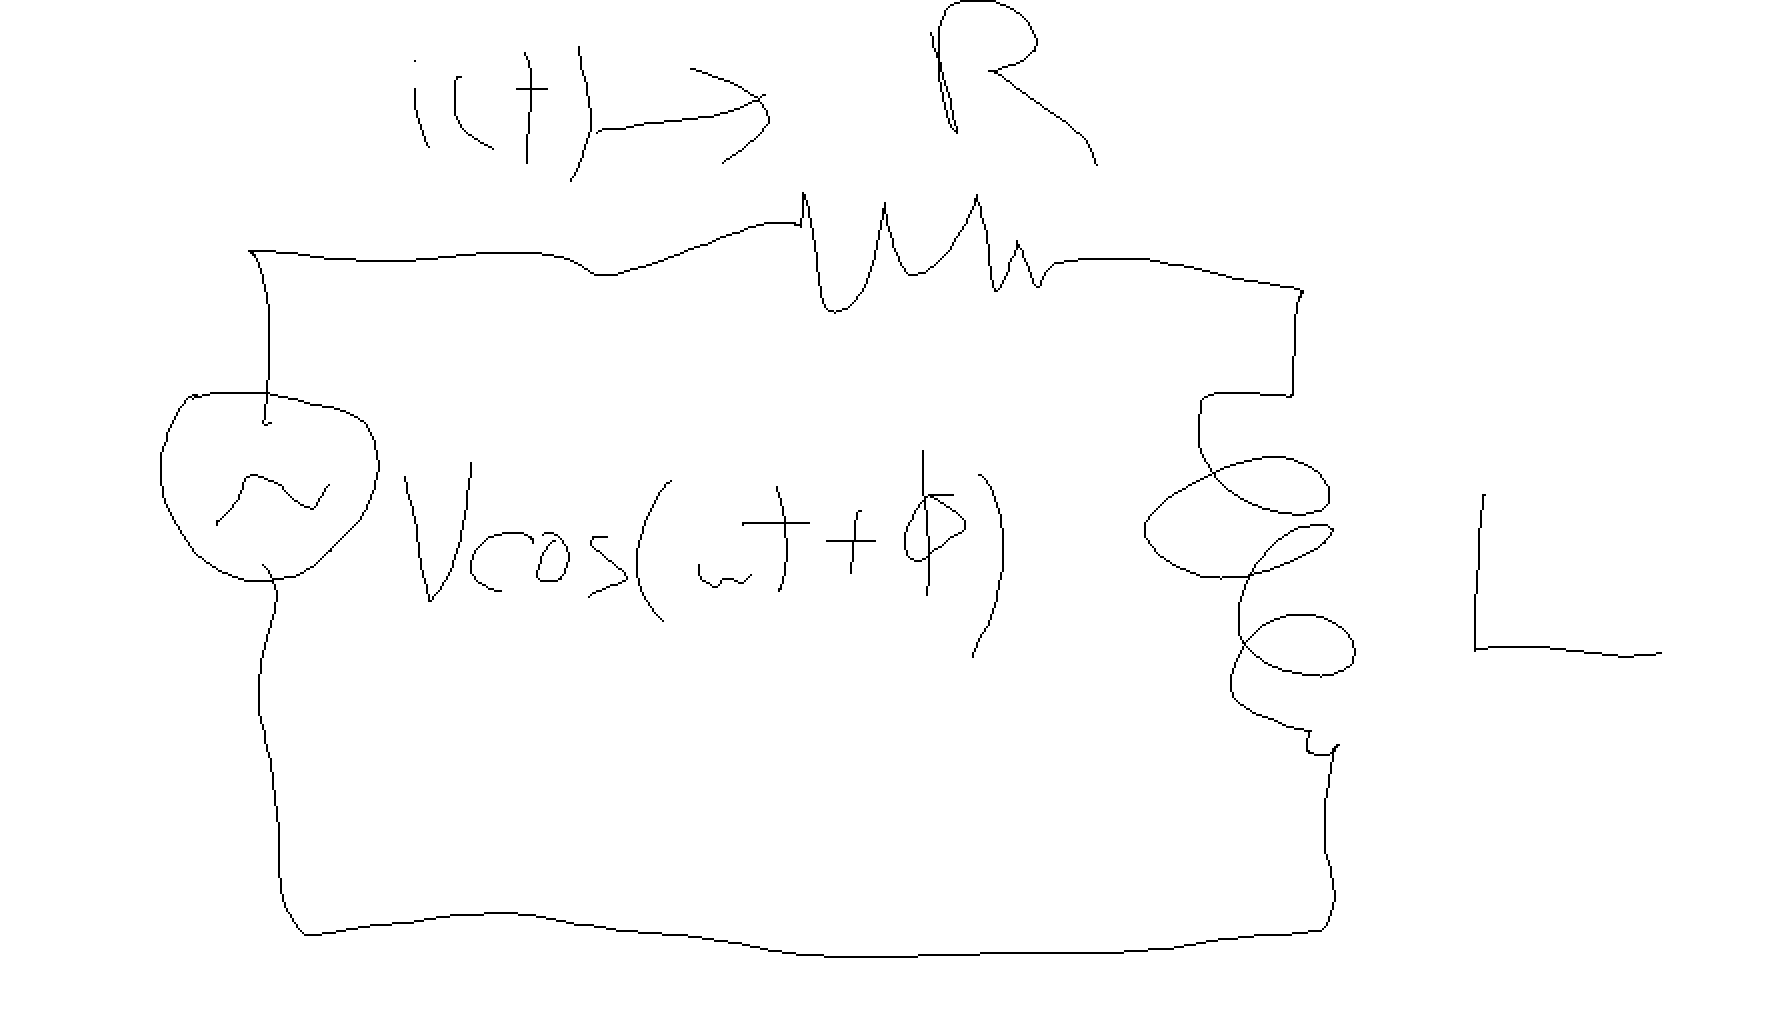
\includegraphics[width=0.8\linewidth]{img/image_2022-09-09-15-23-06.png}
\end{figure}

\begin{equation}
	\begin{split}
		Ri + L \frac{di}{dt} &= V \cos{(\omega t + \phi)}  \\
	\end{split}
\end{equation}


But this is a pain to solve. It can be made simpler by applying phasors

\begin{equation}
	V \cos{(\omega t + \phi)}  = Re\{ Ve^{j(\omega t + \phi)} \}
\end{equation}

Take the real part of $ \hat{I} $:

\begin{equation}
	R \hat{I} + L \frac{d\hat{I}}{dt} = Ve^{j(\omega t + \phi)}
\end{equation}


And therefore by inspection the solution is of format $ \hat{I} e^{j\omega t} $, where $ \hat{I} $ is a phasor. Noting that $ \hat{I} $  contains only amplitude and phase,

\begin{equation}
	\begin{split}
	R \hat{I} e ^{j \omega t} + L \frac{d}{dt}(\hat{I} e^{j \omega t}) &= Ve^{j \omega + \phi} \\
		R \hat{I} + L \hat{I} j \omega  &= Ve^{j \phi} \\
\end{split}
\end{equation}

And now reconstructing:

\begin{equation}
	\begin{split}
		\hat{I} &= \frac{V}{\sqrt{R^2 (\omega L)^2}} e^{j(\omega t + \phi - \tan^{-1}{\frac{wL}{R}})} \\
		 i(t) &= Re \left\{ \hat{I} \right\}   \\
	\end{split}
\end{equation}

And therefore

\begin{equation}
	\hat{I} = \frac{V}{\sqrt{R^2 (\omega L)^2}} \cos{(\omega t + \phi - \tan^{-1}(\frac{wL}{R}))}
\end{equation}


The steps to solving a phasor problem are:\marginnote{Notation: $ Xe^{j\phi} \leftrightarrow X\lfloor\phi $ }
\begin{itemize}
	\item Define phasor: $ V \cos{(\omega t + \phi)} \leftrightarrow V\lfloor\phi $ 
	\item Map $ L, C $ into phasor domain; find impedences
		\begin{itemize}
			\item $ v = L \frac{di}{dt} \leftrightarrow \hat{V} = j \omega L \hat{I} $ 
			\item $ i = C \frac{dv}{dt} \leftrightarrow \hat{V} = \frac{1}{j \omega C }\hat{I} $ 
		\end{itemize}
	\item Do mesh analysis to find $ \hat{I} $; $ \hat{I} = \frac{\hat{V}}{\sum \text{impedances} } $ 
	\item Reconstruct $ i(t) $ from $ \hat{I} $ 
\end{itemize}


\subsection{Lecture 3}

Phasors allow us to solve circuits with multiple sources of differing frequencies.



\begin{figure}[H]
	\centering
	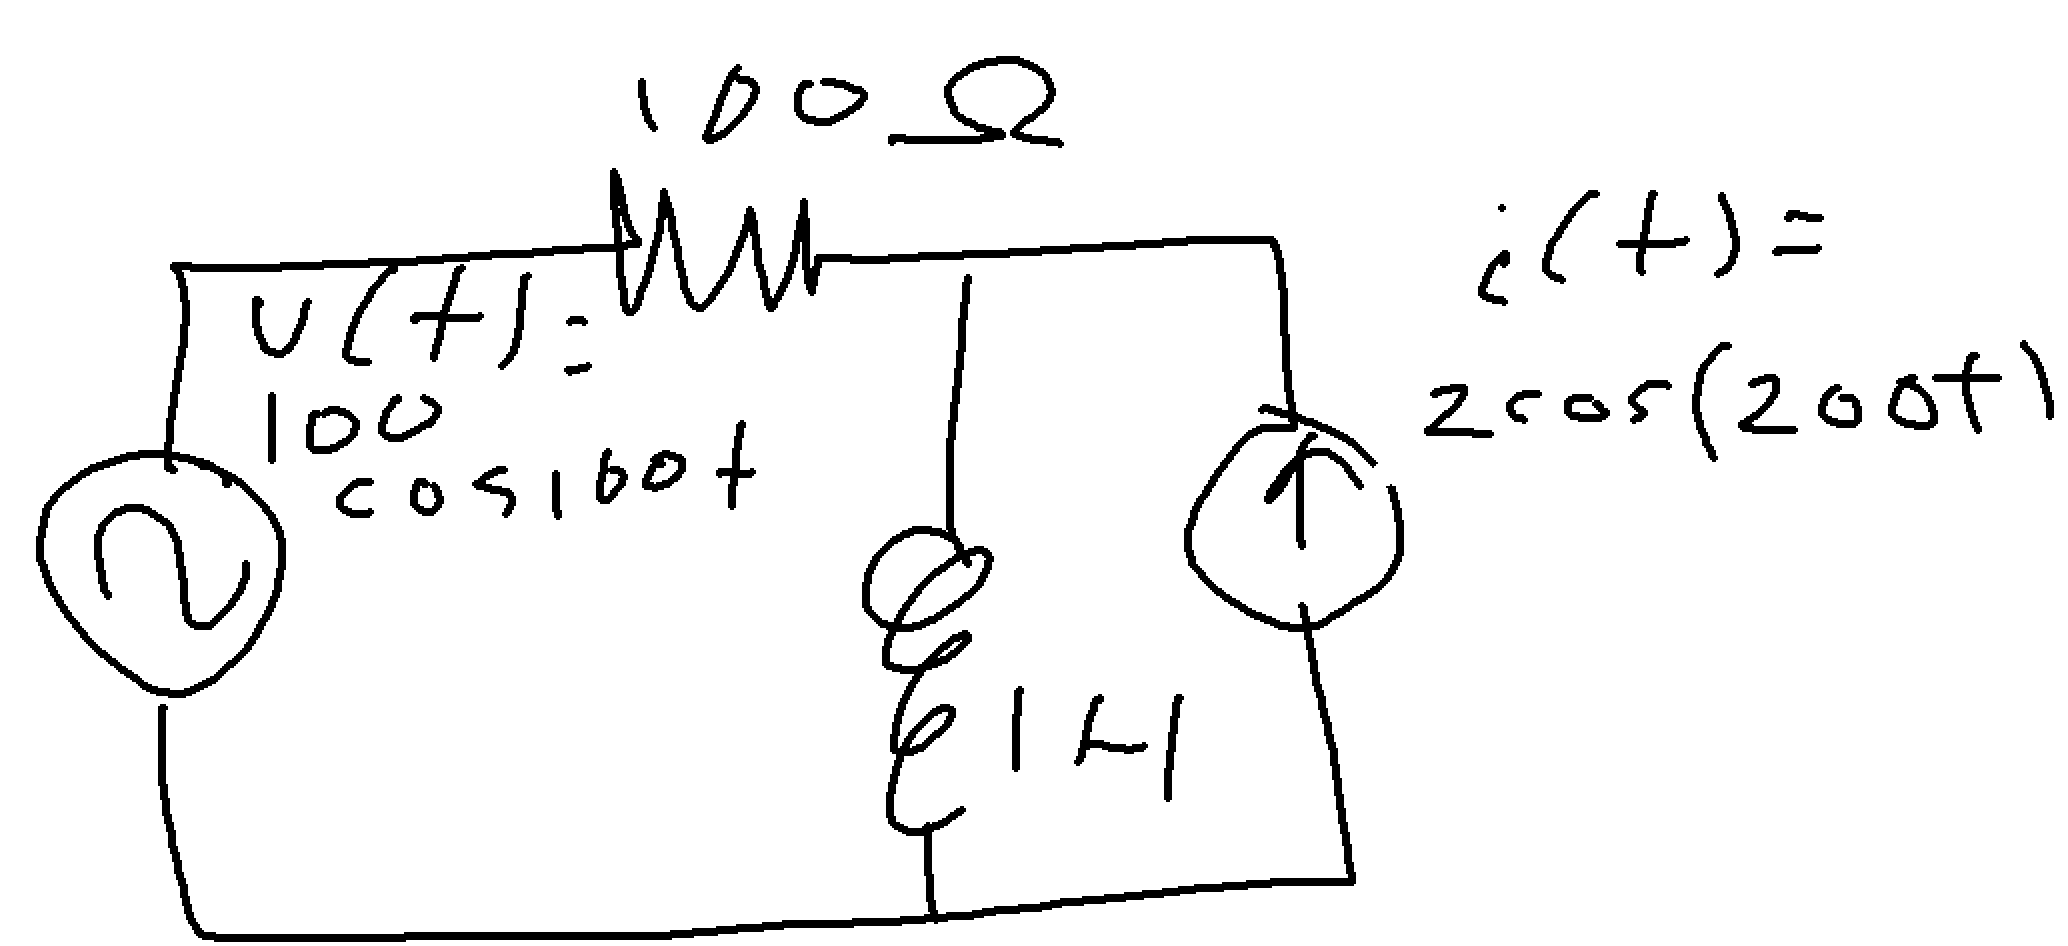
\includegraphics[width=0.8\linewidth]{img/image_2022-09-12-11-19-00.png}
\end{figure}

To find the current $ i(t) $ over the inductor we can find it's response due to the voltage and current sources and then apply superposition.

\begin{itemize}
	\item $ I_1 = \frac{100\lfloor{0}}{1oo + j100} = 0.707\lfloor{-45^o} \rightarrow i_1(t) = 0.707 cos(100t - 45^o) $ 
	\item $ I_2 = \frac{100}{100 + j200} 2\lfloor 0 = 0.894 \lfloor -65^o \rightarrow i_2(t) = 0.894 cos (200t - 63^o)$ 
	\item $ i(t) = i_1(t) + i_2(t) = 0.707cos(100t - 45^o) + 0.894 cos(200t - 63^o) $ 
\end{itemize}

Non-sinusoidal stimulus may be solved by decomposing the signal with Fourier transforms. 
For example, square waves:

\begin{figure}[H]
	\centering
	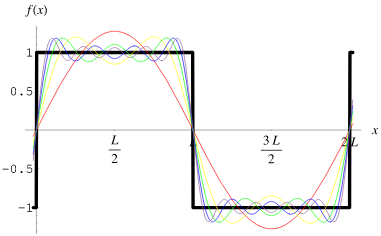
\includegraphics[width=0.8\linewidth]{img/image_2022-09-12-11-28-11.png}
	\caption{square waves with Fourier series superimposed}
\end{figure}

The general form of a Fourier transform is given as:

\begin{equation}
	v_{equiv}(t) = a_o + \sum^\infty_{n=1} a_k cos(nw_ot) + b_k cos(nw_ot)
	\label{eq:349:fourier}
\end{equation}

Where:

\begin{equation}
	\begin{split}
		a_o &=  \frac{1}{T} \int^T_0 v(t) dt \\
		a_k &= \frac{2}{T} \int^T_0 v(t) cos (nw_o t) dt \\
		b_k &= \frac{2}{T} \int^T_0 v(t) sin(nw_o t) dt \\
	\end{split}
	\label{eq:349:fourier_terms}
\end{equation}


Armed with Fourier series and superposition we may now model a non-sinusoidal signal as a superposition of an infinite sum of sources. About half the work can be cut in half by recognizing that $ sin $ lags $ cos $ by $ 90^o $, so


\begin{equation}
	\begin{split}
		a_o &=  \frac{1}{T} \int^T_0 v(t) dt \\
		a_k &= \frac{2}{T} \int^T_0 v(t) cos (nw_o t) dt \\
		b_k &= \frac{2}{T} \int^T_0 v(t) cos(nw_o t - 90^o) dt \\
	\end{split}
\end{equation}

\section{AC Power}

\begin{definition}
	\textbf{Instantaneous Power}: $ p(t) = v(t) \times i(t) [W, \frac{J}{s}]$  

	\begin{example}
		For a circuit with a voltage source, $ v(t) = Vcos(\omega t) $ and a resistor $ \Omega $, $ i(t) = Icos(\omega t) $, $ p(t) = VI cos^2 (\omega t) = \frac{VI}{2}(1+cos(2\omega t))$
	\end{example}
	
\end{definition}

\begin{definition}
	\textbf{Average Power over Cycle}: $ P(t) = \frac{1}{T} \int_o^T p(t) dt = \frac{VI}{2} $  
\end{definition}

If we were to plot the instantaneous power we see that due to the sinusoidal response there are times where $ 0 $ power is supplied.
This will always be true for a single phase power supply; real-world supplies always have multiple phases; this is why computer PSUs always contain a ton of capacitors.


\begin{definition}
	\textbf{Reactive Power}: $ Q $ 


	\begin{figure}[H]
		\centering
		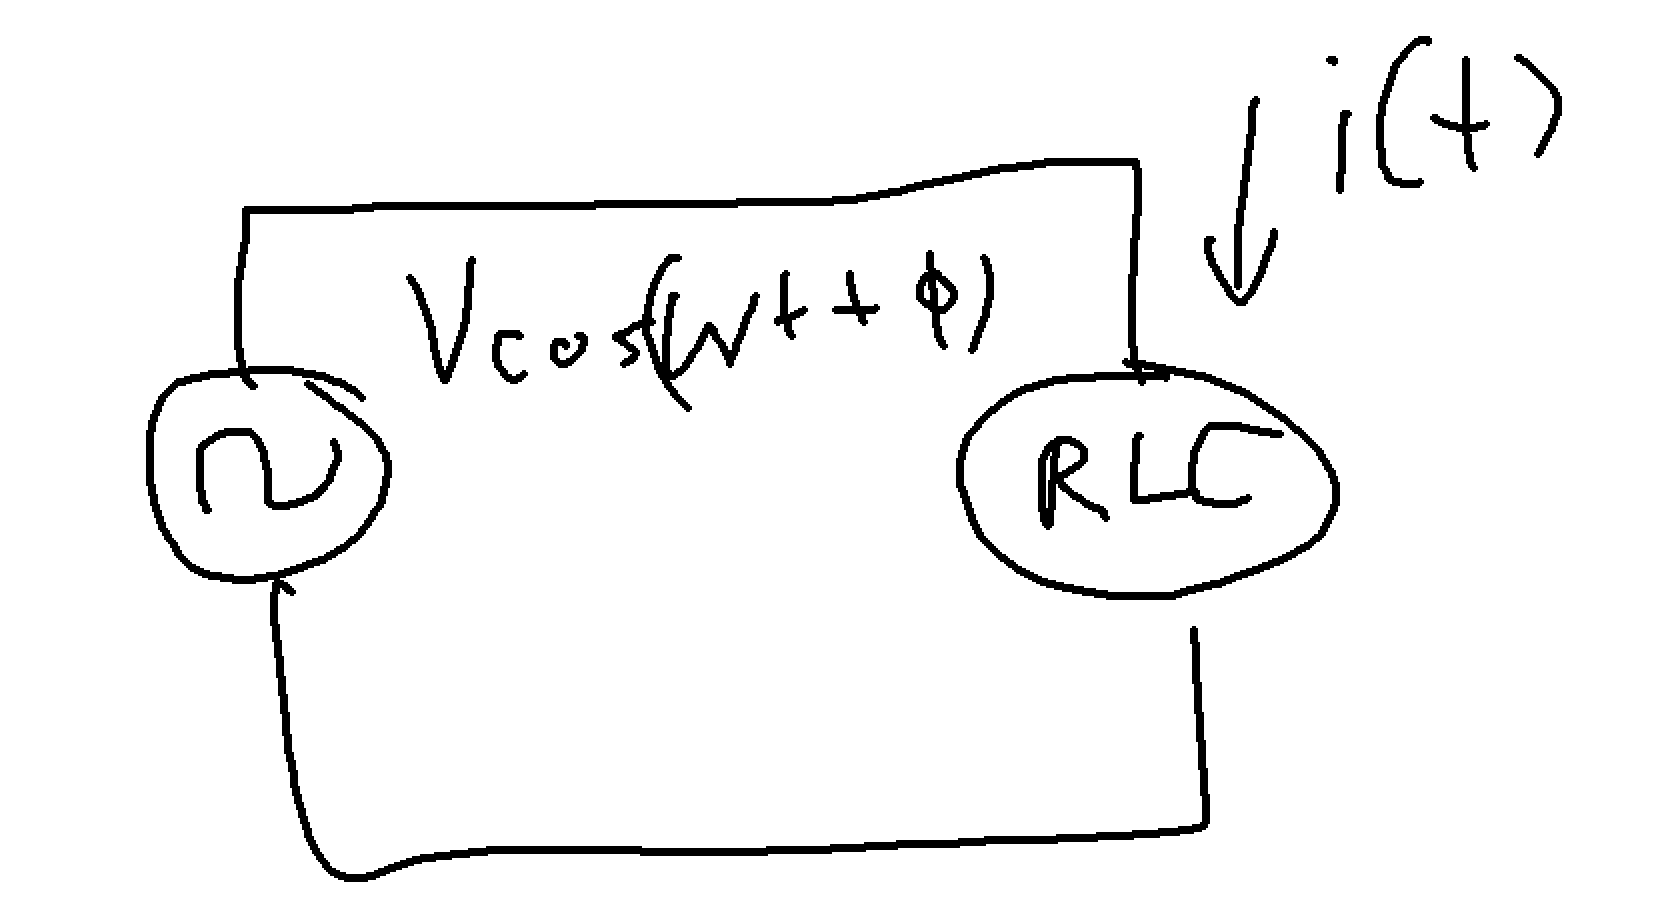
\includegraphics[width=0.8\linewidth]{img/image_2022-09-12-11-49-46.png}
	\end{figure}

	\marginnote{$ \phi = \phi_v - \phi_i $ }

	If $ \phi_i = 0$ and taking $ \phi = \phi_v $,

	\begin{equation}
		\begin{split}
			p(t) &= V\cos(\omega t + \phi) * I \cos(\omega t) \\
					 &= \frac{VI}{2} \cos(\phi) + \cos(2\omega t + \phi) \\
					 &= \underbrace{\frac{VI}{2} \cos(\phi)(1 + \cos(2 \omega t)}_{\text{real power e.g. heat}} 
					 - \underbrace{\frac{VI}{2} (\sin \phi \sin 2 \omega t)}_{\text{stored and released back to source}} \\
		\end{split}
	\end{equation}

	Taking the average power of the reactive power we get 

	\begin{equation}
		P_{avg} = \frac{VI}{2} \cos\phi
	\end{equation}
	Another quantity, reactive power, can be defined with regards to the energy sloshing back and forth:

	\begin{equation}
		Q = \frac{VI}{2} \sin \phi
		\label{eq:349:reactive_power_q}
	\end{equation}
	

\end{definition}

\subsection{Lecture 4}


\begin{definition}
	\textbf{Displacement factor} 

	$ DF \equiv \cos \phi $ 

	Where $ \phi $ is the angle measured from the $ \hat{V} $ to the $ \hat{I} $ phasors.
	A $ DF = 1 $ means the system is transferring the most power possible.

	\begin{itemize}
		\item Lagging DF: $ \phi  $ is -'ve
		\item Leading DF: $ \phi  $ is +'ve'
	\end{itemize}
\end{definition}


We can also write $ P, Q$ from phasors.

\begin{equation}
	\begin{split}
		P  &= \frac{\hat{V} \hat{I}}{2} \cos(\phi_v - \phi_i) \\
			 &= \frac{1}{2} \hat{V} \hat{I} Re\{e^{j\phi_v - \phi_i}\} \\
			 &= \frac{1}{2} Re\{Ve^{j\phi v} \cdot I e^{-j\phi_i}  \} \\
			 &= \frac{1}{2} Re\{\hat{V} \hat{I^*}\} \\
	\end{split}
\end{equation}

\begin{equation}
	\begin{split}
		Q  &= \frac{\hat{V} \hat{I}}{2} \sin(\phi_v - \phi_i) \\
		\vdots \\
			 &= \frac{1}{2} Im \{\hat{V} \hat{I^*}\} \\
	\end{split}
\end{equation}


The expressions for $ Q $  and $ P $ are basically the same so we define a new quantity, complex power, which incorporates both the imaginary and real components.

\marginnote{Reference: Thomas 16.1, 16.2, 16.3}

\begin{definition}
	\textbf{Complex Power} 
	\begin{equation}
		S = \frac{1}{2} \hat{V} \hat{I*} = P + jQ
		\label{eq:349:complex_power}
	\end{equation}
	
\end{definition}


\subsubsection{Root Mean Squared (RMS) Values}


A RMS value measures the average power of a periodic signal. Consider a circuit with an AC voltage source with $ v(t) $ flowing through a resistor. 


The power is:
\begin{equation}
	p(t) = v(t) i(t) = v(t) \frac{v(t)}{R} = \frac{1}{R} v(t)^2
\end{equation}

The average power is therefore

\begin{equation}
	P = \frac{1}{R} \int_0^T v(t)^2 dt
\end{equation}


Evaluating this becomes easier by defining an useful quantity, RMS voltage

\begin{equation}
	v_{rms} = \sqrt{\frac{1}{T} \int^T_0 v(t)^2 dt} 
\end{equation}
	

And using $ v_{rms} $ we get a nice expression for average power,

\begin{equation}
	P = \frac{1}{R} v_{rms}^2
\end{equation}



More generally speaking we can define RMS values of sinusoidal signals

\begin{definition}
	\begin{equation}
		v_{rms} = \sqrt{\frac{1}{2\pi} \int^{2\pi}_0 (\hat{V} \cos wt )^2 dt}  = \frac{1}{\sqrt{2}}  \hat{V}
	\end{equation}
\end{definition}


Plugging this into the expressions for complex power:

\begin{equation}
	S = \underline{V} \cdot \underline{I^*}
\end{equation}

Where $ \underline{V} $, $ \underline{I^*} $ are RMS phasors at a given common frequency.


And more generally yet, the RMS values of non-sinusoidal signals can be found with help of a Fourier expansion


\begin{definition}
	Let $ v(t) = \hat{v}_0 + \hat{v}_1 \cos(wt+\phi_1) + \ldots $ 

	Then,


	\begin{equation}
		v_{rms} = \sqrt{\hat{v}^2 + \frac{\hat{v}_1}{\sqrt{2} }^2 + \frac{\hat{v}_2}{\sqrt{2} }^2 \ldots }   = \sqrt{v_0^2 + \sum^\infty_{n=1} (\frac{V_m^2}{2})} 
	\end{equation}

	And if $ V_m $ is the $ rms $ value,

	\begin{equation}
		v_{rms} = \sqrt{v_0^2 + \sum^\infty_{n=1} V_m^2} 
	\end{equation}
	

\end{definition}

One thing to watch out for is that we could have a system with high voltage but near-zero current transferring little to no power. 
To account for this we look at the power factor `PF'

\begin{definition}
	\textbf{Power Factor} 
	\begin{equation}
		PF \equiv \frac{\text{average power}}{\text{rms voltage} \cdot  \text{rms current}}
	\end{equation}
\end{definition}

For a sinusoidal $ V, I $:


\begin{equation}
	\begin{split}
		PF &= \frac{\frac{1}{2} \hat{V} \hat{I} \cos \phi}{  \frac{\hat{V}}{\sqrt{2} } \cdot  \frac{\hat{I}}{\sqrt{2} }  }  \\
		 &=  \cos\phi\\
	\end{split}
\end{equation}


If signals are not harmonics $ PF = DF $. This can be a source of confusion. 


For non-sinusoidal systems this becomes more difficult because, unlike pure signals, they may contain harmonics.
In these systems either $ V, I $, or both may contain harmonics. 
Generally in household power $ V $ is clean but $ I $ contains harmonics.


The effect of harmonics in currents is that $ I_{\text{harmonics}} $ causes a higher $ I_{rms} $; there is more current but no higher power!
This reduces $ PF $ and causes $ PF < DF $.


To summarize, 

\begin{itemize}
	\item In ideal systems, $ PF = DF $ if all $ V $ and $ I $ are at one frequency.
	\item $ PF = 1 $ means no energy sloshing between load and source.
\end{itemize}

Harmonics are bad because they reduce the usefulness of the system
There are very tight standards for how many harmonics one is allowed to inject into the system via generators or loads.
See: textbook 16.6










% 349 END

\part{ECE352: Computer Organization}

\marginnote{Taught by Prof. Andreas Moshovos}
\section{Admin stuff}
\subsection{Lecture 1}



\begin{itemize}
	\item Lecture recordings on \href{https://tinyurl.com/2jthyk8k}{YouTube}
	\item Online notes: \href{https://www.eecg.utoronto.ca/~moshovos/ECE352-2022}{https://www.eecg.utoronto.ca/~moshovos/ECE352-2022/}
	\item Course will cover the following:
	 \begin{itemize}
	 	\item C to assembly
		\item How to build a processor that works
		\item Intro to processor optimizations
		\item Peripherals
		\item OS support (Maybe)
		\item (Maybe) Arithmetic circuits
		\item Use NIOS II and cover a little bit of RISC-V
	 \end{itemize}	
\end{itemize}



\subsubsection{Mark breakdown}

\begin{itemize}
	\item Labs 15\%
	\item project 5\%
	\item midterm  30\%
	\item Final 50\%
	\item All exams will be open notes/book/whatever except another person/service helping you.
\end{itemize}

\section{Preliminary}
\subsection{Lecture 2: Using binary quantities to represent other things}

Computers can represent information in bits; 0/1. 
Though they don't necessarily know or care what bits are, we may assign our own arbitrary meaning to them -- usually numbers with the help of positioning; the LSB represents $ 2^0 $ and so forth.

C types \marginnote{Or, just \texttt{\#include <stdint.h>}...}
	\begin{itemize}
		\item int: 32b (word)
		\item char: 8b (byte)
		\item short: 16b (half word)
		\item long: 32b (word)
		\item long long: 64b
	\end{itemize}

Signed numbers may be represented in a number of ways.
\begin{itemize}
	\item Sign bit (make MSB represent positive or negative numbers and then the remaining $ n-1 $ bits represent the number. Con: hardware impl sucks because requires if/else
	\item Two's complement \sidenote{Flip bits, add one. Intuition; in 3 bit system, adding 7 to 1 would result in 8 which would get truncated to 0.}. Pro: only need to implement adders on hardware and then negative numbers will work just like any other except must be interpreted differently. Positive numbers would always start with a $ 0 $ and negatives would start with $ 1 $. So the range of possible values becomes $ -(2^{n-1}-1), +2^{n-1}-1$ 
\end{itemize}

Adding together binary numbers can also cause overflow; $ (A+B) \ge A, (A+B) \ge  B $ may not always be true.
Also, when we work with these types we always use all the bits. This has implications when working with values of different lengths.

\begin{itemize}
	\item \texttt{char b = -1}  \texttt{(1111 1111))}
	\item \texttt{short int c = -1}  \texttt{(0000 0000 0000 0001))}
	\item \texttt{a = b + c} \texttt{0000 0001 0000 0000 } 
	\item In order to deal with this we must \texttt{cast} the \texttt{char} to a \texttt{short int}. This is done via sign extension which prepends $ 0 $s or $ 1 $s \sidenote{two's complement} to the \texttt{char} so that math can be done on it.
\end{itemize}


\subsubsection{Floating Point Numbers}


Whereas fixed point numbers i.e. $ \$5.25 $ can be represented just as how an integer would be represented but with the understanding that the user would interpret it as having a decimal point somewhere that indicates the position of $ 2^0 $.
This decimal point would be the same for all numbers of that type, i.e. we could have a six bit number that has places $ 2^2 2^1 2^0 2^{-1} 2^{-2} $ 
This is common in embedded systems and how it is formatted isn't super clearly standardized.

\begin{lemma}
	Reference: \href{https://www.eecg.utoronto.ca/~moshovos/ECE352-2022/00.practice/What\%20Every\%20Computer\%20Scientist\%20Should\%20Know\%20About\%20Floating-Point\%20Arithmetic.htm}{What Every Computer Scientist Should Know About Floats}
\end{lemma}





\begin{definition}
	\textbf{IEEE 754 Floating Point}

	This is a single precision 32 bit float

	\begin{equation}
		\texttt{S  EEEEEEEE  MMMM MMMM MMMM MMMM MMMM MMM}
	\end{equation}
	

	The most significant \texttt{S} bit is the sign bit, bits 30 through 23 \texttt{E} form the exponent which is an unsigned integer, and 22 through 0 form the (\texttt{M})antissa. The number being represented can be found using the following:

	\begin{equation}
	(-1)^S \times 2 ^ {(E-127)} \times 1.\text{Mantissa}
		\label{eq:352:float32_eq}
	\end{equation}

	\begin{example}
		For example, given the following float:
		\begin{equation*}
			1\quad10000001\quad10000000000000000000000
		\end{equation*}
		
		So S = 1, E = 10000001 = 129 and Mantissa = 10000000000000000000000.
		The number is therefore

		\begin{equation}
			(-1^1) \times 2^{(129-127)} \times 1.10000000000000000000000 = -6.0
		\end{equation}
	\end{example}


	IEEE754 also defines 64 bit floating-point numbers. They behave the same except for now having an 11 bit exponent, the bias being 2047\mn{instead of 126}, and the mantissa having 52 bits\marginnote{In \texttt{c}, \texttt{float} is a 32 bit float and \texttt{double} is 64}.


	A few special cases are also available to represent other quantities

	\begin{itemize}
	\item If E=0, M non-zero, value=$(-1)^S \times 2^{-126} \times 0.M$ (denormals)
		\item If E=0, M zero and S=1, value=-0
		\item If E=0, M zero and S=0, value=0
		\item If E=1...1, M non-zero, value=NaN 'not a number`
		\item If E=1...1, M zero and S=1, value=-infinity
		\item If E=1...1, M zero and S=0, value=infinity
	\end{itemize}

	Floating-point numbers are inherently imprecise. Addition and subtract are inherently lossy; the mantissa window may not be large enough to capture the decimal points. Multiplication and division just creates a ton of numbers.
	\marginnote{There are more floating point formats introduced by nvidia and google such as a half-precision or 8-bit float designed to reduce memory use for machine learning}

	Converting real numbers to IEEE754 floats, here using 37.64 as an example, can be done as follows
	\begin{itemize}
		\item Repeatedly divide the part of the number $ >0 $ by $ 2 $ and get the remainders, i.e. 37/2 = 18, rem = 1 -> 18/2 = 0, rem = 0 -> 4/ 2 = 2, rem = 0, 2/2 = 1, rem = 0, 1/2 = 0, rem = 1; E = 100101
		\item Do the same for the part of the number past the decimal, but multiplying by two and checking if > 1: 0.64 * 2 = 1.28 -> 1, 0.28 * 2 = 0.56 -> 0, 0.56 * 2 = 1.12 -> 1 ... and so forth. At some point we will hit a cycle but we'll just take the $ N_{\text{mantissa}} $ of digits.
	\end{itemize}

	So the full number is $  0 1000 0100 0010 1101 0001 1110 1011 111 $
\end{definition}


\section{NIOS II}


\subsection{Lecture 3: Behavioural Model of Memory}


Computers can be described as a set of units, each of which interact with each other and the outside world in a specified way.
For example, modern computers tend to have memory units, processing units, display units, and so forth.
Each unit has a set of inputs and outputs, and a set of rules that govern how the unit behaves.
This gives the manufacturer flexibility in how they want to implement a unit, as long as the unit behaves as specified.
When designing these operational units it is important to strike a balance between functionality and specificity; if the unit is too specific it will be difficult to implement, but if it is too general it will be difficult to use.

\marginnote{\textbf{Specification} is the description of what an unit should do, and \textbf{implementation} is how it actually does it. For example, an \texttt{OR} gate can be specified as a truth table and then implemented via transistors or a person in a box.}

\subsubsection{Memory}
Memory is a unit that stores information and is usually represented as a vector of elements, usually a byte (8 bites).
Each element, or memory location, contains a binary quantity and has an associated \textit{address}.
The address is a number that uniquely identifies the location of the element in the vector, and is \textbf{permanently fixed} at time of manufacture.
Most systems are byte-addressable, meaning that there is an unique address for each byte in the memory.
The collection of all addresses is called the \textbf{address space} of the memory, which is typically a power of two.
Modern systems tend to be 32 or 64 bit, meaning that the address space is $ 2^{32} $ or $ 2^{64} $ elements long.

For each memory location there there are two operations available
\begin{itemize}
	\item \textbf{Read}: Read the value stored at a given address
	\item \textbf{Write}: Write a value to a given address
\end{itemize}


Typical memory behaviour models define that the order of memory operations matters, i.e. 

\begin{enumerate}
	\item \texttt{store 0x10, 0xf0} 
	\item \texttt{store 0x20, 0xf0} 
\end{enumerate}

We would see that \texttt{0xf0} contains the value \texttt{0x20} and not \texttt{0x10} due to the sequential execution model.
Memory that adheres to the sequential model offers operations that are \textbf{atomic}; the operations are performed on its own with no interaction or overlap with anything else.



\begin{figure}[H]
	\centering
	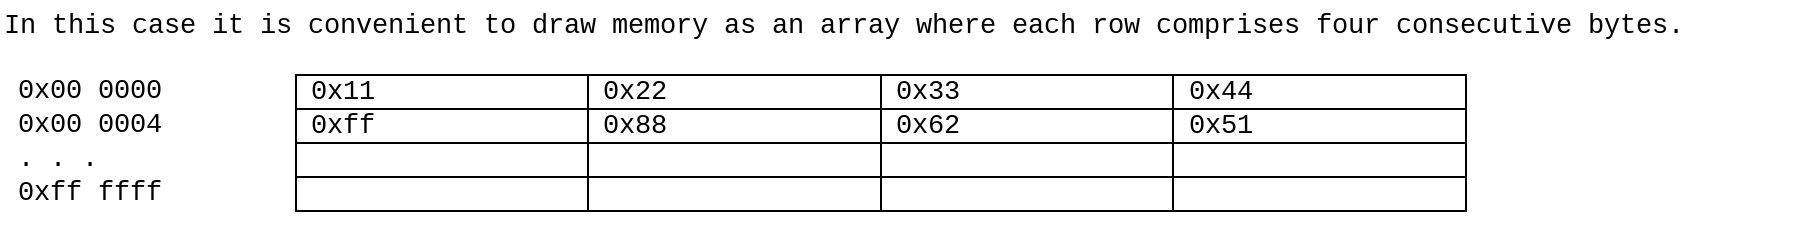
\includegraphics[width=\linewidth]{img/image_2022-09-16-02-10-27.png}
\end{figure}

Systems are generally also addressable by words, halfwords, and bytes.
Different architectures have different constraints on allowing unaligned access\sidenote{Aligned access only means to allow [only] reads or writes for a data size i.e. halfword to an address divisible by the size of said data type. For example an longword access on our development board would be at an address divisible by $ 4 $}

\textbf{Endianness} refers to the order in which bytes are stored in memory. Though some processors are big-endian, most modern processors are little-endian. The NIOS II used for this course is little-endian. 

\begin{figure}[H]
	\centering
	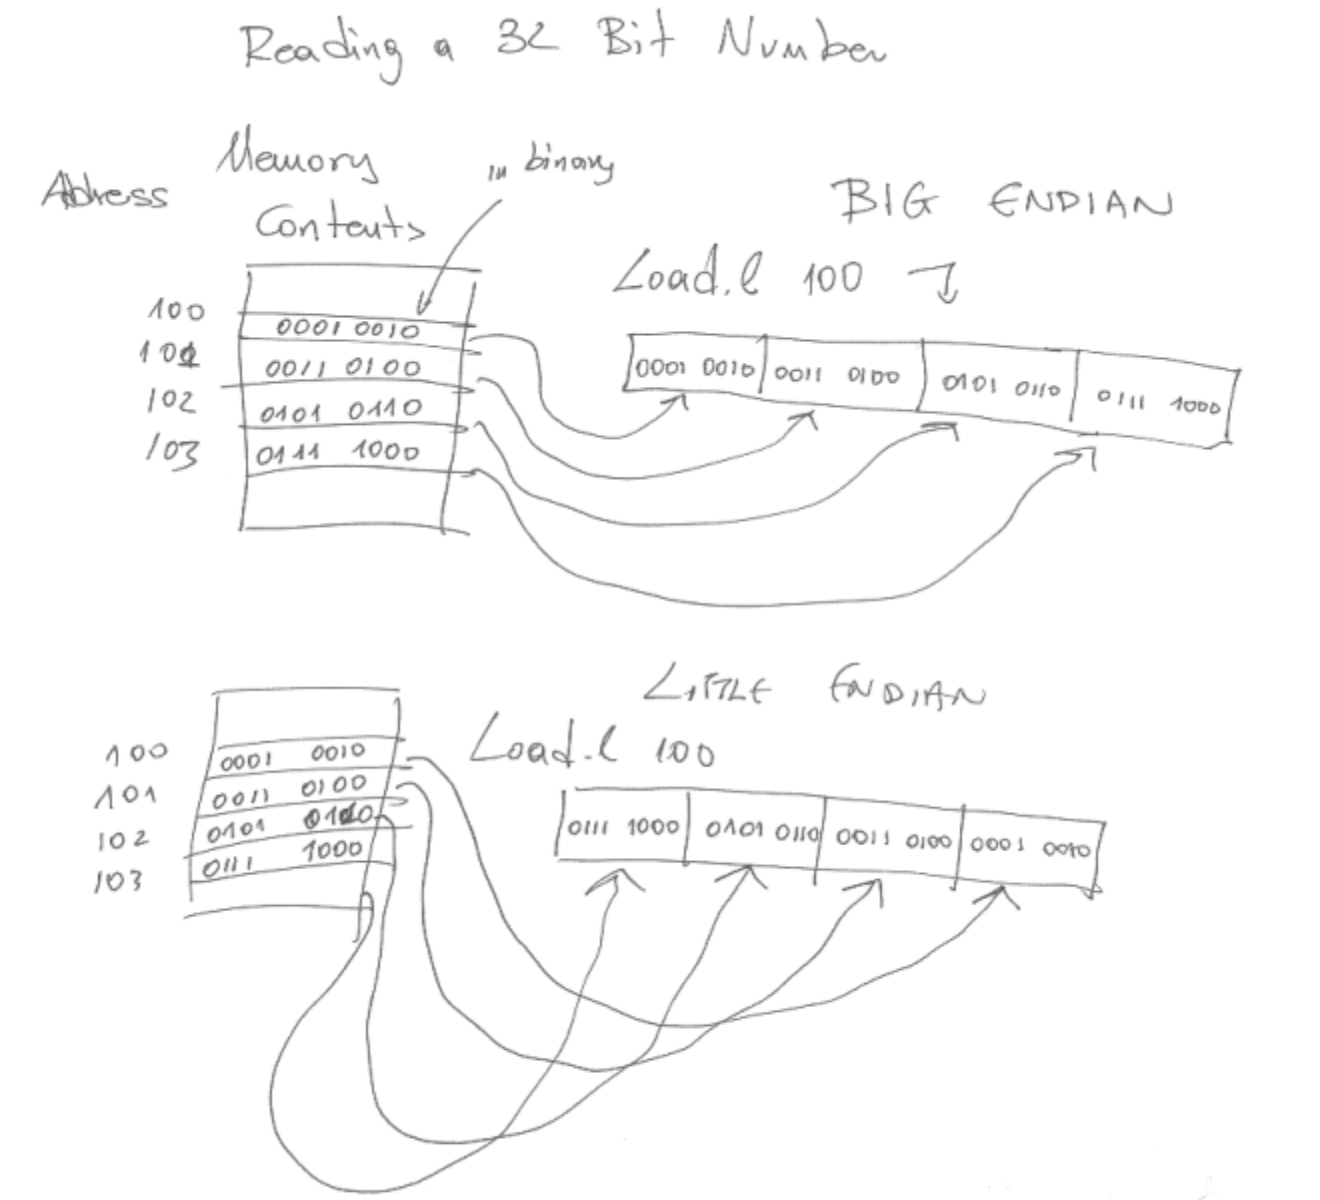
\includegraphics[width=0.8\linewidth]{img/image_2022-09-16-02-16-30.png}
\end{figure}

\subsubsection{Physical Interface}

What physical interfaces would be necessary to implement this behavioural model? 

Given a summary of requirements as follows:

\begin{enumerate}
	\item Read and write operations
	\item Addressable by byte, word, longword
	\item 24 bit address
	\item 32 bit for writing
	\item 32 bit for reading
	\item signal for do nothing
\end{enumerate}


A single bit signal can be used to indicate whether the memory is reading or writing, and a two bit signal can be used to specify if we're interested in addressing by byte, word, or longword.
The address is 24 bits, so we need 24 address lines.
As for reading/writing data, we have the option of having two 32 bit data lines, or multiplexing a single 32 bit line.
A single bit signal can be used to indicate to do nothing or not. \marginnote{The use of a single bit signal to indicate `do nothing' is necessary because a physical device won't be able to change all signals instantaneously, so we use it to tell the memory to wait until these transient effects die off}

One way of multiplexing the data lines is to use a tri-state buffer, which is a buffer that can be enabled or disabled.
When enabled, the buffer acts as a normal buffer, but when disabled, the output is disconnected from the input.
On the other hand this means that our memory chip would not support simultaneous reads or writes.




\begin{figure}[H]
	\centering
	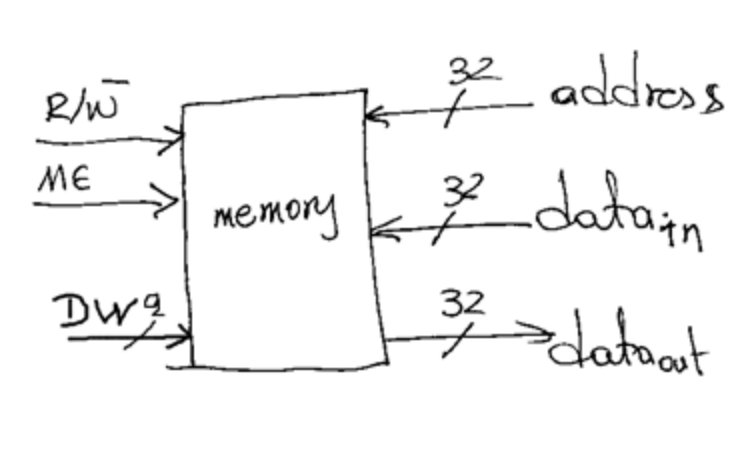
\includegraphics[width=0.8\linewidth]{img/image_2022-09-16-02-18-16.png}
\end{figure}

\subsection{Lecture 4: NIOS II Programming Model}

The NIOS II assumes a \texttt{32-bit} address space where each address holds a single byte.
Each byte is addressable, and three data types are supported. Halfword and word accesses must be aligned.

\begin{itemize}
	\item \textbf{Byte}: 8 bits
	\item \textbf{Halfword}: 16 bits
	\item \textbf{Word}: 32 bits
\end{itemize}

The NIOS II also has a set of registers

\begin{itemize}
	\item 32 general purpose 32 bit registers
		\begin{itemize}
			\item \texttt{r0} is always zero\marginnote{Many operations can be synthesized using another operation involving zero, i.e. assignment \texttt{A=B} can be implemented as \texttt{A = B + 0} }
		\end{itemize}
	\item 6 control registers, 32 bits each
	\item Program counter (PC), 32 bits
\end{itemize}

There are certain conventions for the use of registers, which are as follows:
\begin{figure}[H]
	\centering
	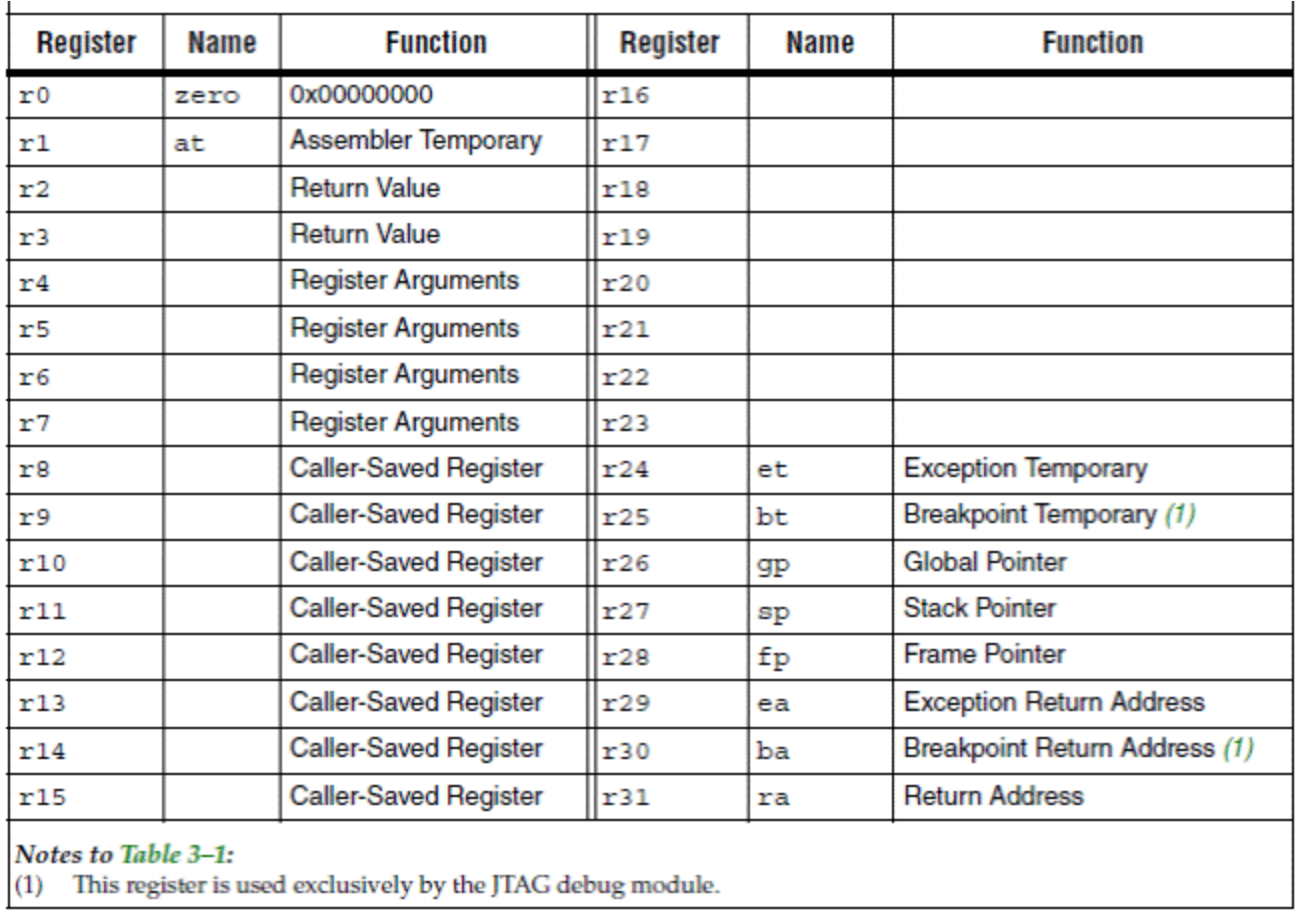
\includegraphics[width=0.8\linewidth]{img/image_2022-09-16-17-17-34.png}
\end{figure}

\subsubsection{Adding Two Numbers}
As an exercise, let's see how we can implement the following piece of code in NIOS II assembly

\begin{listing}[H]
\begin{minted}{c}
unsigned int a = 0x00000000;
unsigned int b = 0x00000001;
unsigned int c = 0x00000002;

a = b + c;
\end{minted}
\end{listing}


\textbf{Register-only version} 

\marginnote{\texttt{addi} stands for `add intermediate', the only difference being that the second operand is a number. It is used to set a constant}

\begin{listing}[H]
\begin{minted}{gas}
addi r9, r0, 0x1
addi r10, r0, 0x2
add r9, r10, r11
\end{minted}
\end{listing}

In general, most instructions take the form of \texttt{operation destination, source1, source2}.


Breaking it down even further we can see that these assembly instructions actually perform a number of steps

\begin{listing}[H]
\begin{minted}{gas}
addi r9, r0, 0x1
	; 1. read r0
	; 2. Add value read in step 1 with 0x1
	; 3. Write result of step 2 to r9
	; 4. increment PC to next instruction
addi r10, r0, 0x2
	; 1. read r0
	; 2. Add value read in step 1 with 0x2
	; 3. Write result of step 2 to r10
	; 4. increment PC to next instruction
add r9, r10, r11
	; 1. read r10
	; 2. read r11
	; 3. Add values read in steps 1 and 2
	; 4. Write result of step 3 to r8
	; 5. increment PC to next instruction
\end{minted}
\end{listing}


What about 32 bit constants? An unfortunate quirk is that \texttt{addi} only supports 16 bit constants, so we need to use \texttt{ori} to set the upper 16 bits of the register.


\begin{listing}[H]
\begin{minted}{gas}
movhi r9, 0x1122
	; Sets the upper 16 bits of r9 to 0x1122
	; and the lower 16 bits to zero
ori r9, r9, 0x3344
	; bitwise OR the value in r9 with 0x3344
	; which will set the lower 16 bits to 0x3344
\end{minted}
\end{listing}

This is a PITA so NIOS II offers a few pseudo-instructions to make this easier




\begin{listing}[H]
\begin{minted}{gas}
movi rX, Imm16
	; sets rX to the sign-extended (signed) 16 bit immediate
movui rX, Imm16
	; sets rX to a zero-extended unsigned 16 bit immediate
movia rX, Imm32
	; sets rX to a 32 bit immediate
\end{minted}
\end{listing}

{\let\thefootnote\relax\footnote{
	\begin{itemize}
		\item Footnote1: \texttt{movia} does not use the \texttt{movhi} and \texttt{ori} instructions to create a 32-bit immediate but rather a \texttt{movhi} and a \texttt{addia}.
\texttt{addi}  will sign extend it's 16-bit field so some adjustment might be needed for whatever is being passed to \texttt{movhi}.
		\item Footnote2: movhi r9, \%hi(0x11223344) is equivalent to movhi r9, 0x1122. Ori r9, \%lo(0x11223344) is equivalent to ori 9, 0x3344. That is, \%hi(Imm32) returns the upper 16-bits of Imm32 and \%lo(Imm32) the lower 16 bits.
		\item Footnote3: movhi r9, \%hiadj(0x11223344) followed by addi r1, \%lo(0x11223344) is the correct way of creating a 32-bit immediate using movhi and addi. \%hiadj(Imm32) returns the upper 16 bits of the immediate  as-is or incremented by 1 if bit 15 is 1. Think why this is necessary based on footnote 1.
		\item Footnote4: \%hi(), \%lo(), and \%hiadj() are macros supported by the assembler. They are not NIOS II instructions. They get parsed during compile time. 
	\end{itemize}
}}


\subsubsection{Adding two numbers using memory}

NIOS II is a load/store architecture which means that all data manipulation happens only in registers.


\begin{listing}[H]
\begin{minted}{gas}
; read b from memory into r9
movhi r11, 0x0020
ori   r11, r11, 0x0004
ldw   r9, 0x0(r11)

; read c from memory into r10
movhi r11, 0x0020
ori   r11, 0x0008
ldw   r10, 0x0(r11)

; add, then store into r8
add   r8, r9, r10

; store r8 into memory
movhi r11, 0x0020
ori   r11, r11, 0x0000
stw   r8, 0x0(r11)
\end{minted}
\end{listing}


The new instructions introduced here are


\begin{listing}[H]
\begin{minted}{gas}
ldw rX, Imm16(rY) ;; 'load word' from memory
;; rX, rY registers, Imm16 is a 16 bit immediate
;; TLDR; Rx = mem[rY + sign-extended(Imm16)]
; 1. read rY
; 2. sign-extend Imm16 to 32bits
; 3. adds the result of step 1 and 2
; 4. reads from memory a word (32 bit) using the result of step 3 as the address
; 5. write the result of step 4 to rX
\end{minted}
\end{listing}

\begin{listing}[H]
\begin{minted}{gas}
stw rX, Imm16(rY) ;; 'store word' to memory
;; rX, rY registers, Imm16 is a 16 bit immediate
;; TLDR; mem[rY + sign-extended(Imm16)] = rX
; 1. read rY
; 2. sign-extend Imm16 to 32bits
; 3. adds the result of step 1 and 2
; 4. write to memory rX using the result of step 3 as the address
\end{minted}
\end{listing}

This can be simplified using the \texttt{movia} macro

\begin{listing}[H]
\begin{minted}{gas}
movia r11, 0x200004
ldw   r9, 0x0(r11)
movia r11, 0x200008
ldw   r10, 0x0(r11)
add   r8, r9, r10
movia r11, 0x200000
stw   r8, 0x0(r11)
\end{minted}
\end{listing}


In this lecture so far we have seen three addressing modes

\begin{enumerate}
	\item Register addressing, i.e. \texttt{rX} 
	\item Immediate addressing, i.e. \texttt{Imm16}
	\item Register indirect addressing with displacement, i.e. \texttt{Imm16(rY)}. This is how we calculate the referenced memory address. Register indirect refers to using a register's value to refer to memory, and `displacement' refers to adding a constant prior to using the register value to access memory. Register indirect addressing is where we use a displacement of 0.
\end{enumerate}


We can exploit register indirect addressing with displacement.

\begin{listing}[H]
\begin{minted}{gas}
movhi r11, 0x0020
ori   r11, r11, 0x0004
ldw   r9, 0x0(r11)
;; can be replaced with
movhi r11, 0x0020
ldw r9, 0x4(r11)
\end{minted}
\end{listing}

Note that the value of \texttt{r11} does not change since the subsequent operations use an offset to that value.

Generally when we want to read memory from \texttt{A} we can use

\begin{listing}[H]
\begin{minted}{gas}
movhi r11, (upper 16 bits of A)
ori   r9, r11, (lower 16 bits of A)
\end{minted}
\end{listing}


Care must be taken when the 16th bit of \texttt{A}  is 1 since the addition that \texttt{ldw} performs will sign extend it to be a negative number, i.e. 

\begin{listing}[H]
	\begin{minted}{gas}
movhi r11, 0x0020
ldw r9, 0x8000(r11)
;; this is incorrect because
;; will extend to 0xFFFF8000, which would result
;; in a final address of 0x001F800
\end{minted}
\end{listing}


This is where the macros \texttt{\%hiadj(Imm32)}  and \texttt{\%lo(Imm32)} come in handy, since they will add 1 to the values if bit 15 of Imm32 is 1. 
This results in code that looks like this:


\begin{listing}[H]
	\begin{minted}{gas}
movhi r11, %hiadj(0x208000)
ldw r9, %lo(0x2080000)(r11)
;; will extend to 0xFFFF8000, which would result
;; in a final address of 0x001F800
\end{minted}
\end{listing}





% 352 END

\part{ECE355: Signal Analysis and Communication}

\marginnote{Taught by Prof. Sunila Akbar}

\section{Admin and Preliminary}
\subsection{Lecture 1}
\begin{itemize}
	\item  CT and DT signals
	\item A ton of LTI (Linear time invariant) systems
	\item Processing of signals via LTI systems
	\item Fourier transforms
	\item Sampling
\end{itemize}
\subsubsection{Mark Breakdown}

\begin{table}[H]
	\centering
	\caption{Mark Breakdown}
	\begin{tabular}{|c|c|}
		\hline
		Homework & 20 \\
		MT1 & 20 \\
		MT2 & 20 \\
		Final & 40 \\
		\hline
	\end{tabular}
\end{table}

% \marginnote{HW is due two weeks after it is assigned}

\begin{itemize}
	\item Continuous enclose in (), independent is $ t $ 
	\item Discrete: enclose in [], independent is $ n $ 
\end{itemize}


\marginnote{In many systems we are interested in power and energy of signals over an infinite time interval; $ -\infty < \{ t, n \} < \infty$ }

\begin{theorem}
	\textbf{Energy for Complex Signals} 

	\begin{equation}
		E_{[t_1, t_2]} = \int_{t_1}^{t_2} \abs{x(t)}^2 dt
		\label{eq:355:energy_CT}
	\end{equation}

	\begin{equation}
		E_{[t_1, t_2]} = \sum_{n=n_1}^{n_2} \abs{x(t)}^2 dt
		\label{eq:355:energy_DT}
	\end{equation}

	\textbf{Average Power for Complex Signals} 

	\begin{equation}
		P_{avg, [t_1, t_2]} = \frac{1}{t_2 - t_1} \int_{t_1}^{t_2} \abs{x(t)}^2 dt
		\label{eq:355:power_avg_CT}
	\end{equation}

	\begin{equation}
		P_{avg, [t_1, t_2]} = \frac{1}{n_2 - n_1 + 1} \sum_{n=n_1}^{n_2} \abs{x(n)}^2
		\label{eq:355:power_avg_DT}
	\end{equation}
		
\end{theorem}


\section{Transformations}

\subsection{Lecture 2}
Most of this lecture was review. When applying transforms just note to always scale, \textit{then} shift, i.e.

\begin{enumerate}
	\item $ y(t) = x(\alpha t) $ 
	\item $ y(t) = x(\alpha t+\frac{\beta}{\alpha}) $ 
\end{enumerate}


\begin{definition}
	\textbf{Fundamental Period} 


	\begin{equation}
		x_t = x(t+ mT), m \in \mathbb{Z}
		\label{eq:355:fundamental_period}
	\end{equation}

	The fundamental period, $ T_o $  is the smallest positive value of $ T $ for which this holds true
\end{definition}

\begin{definition}
	\textbf{Even signals} 
	\begin{equation}
		x(t) = x(-t)
		\label{eq:355:even_signal}
	\end{equation}
\end{definition}

\begin{definition}
	\textbf{Odd signals} 
	\begin{equation}
		x(t) = -x(t)
		\label{eq:355:odd_signal}
	\end{equation}
\end{definition}


\begin{theorem}
	Any signal can be broken into an even and odd component

	\begin{equation}
		\begin{split}
			x(t) &= Ev \left\{ x(t) \right\} = \frac{1}{2} \left[ x(t) + x(-t) \right]  \\
			x(t) &= Od \left\{ x(t) \right\} = \frac{1}{2} \left[ x(t) + -x(-t) \right]  \\
		\end{split}
		\label{eq:355:even_odd_decomposition}
	\end{equation}
\end{theorem}


\subsection{Lecture 3}

Again, most of this lecture was review from the waves portion of PHY293 from last year or some other course prior.



A complex exponential and sinusoidal system can be represented as 
\begin{equation}
	x(t) = C e^{at}
\end{equation}

Where $ C, a $ are complex numbers.

Two cases may occur.

If $ a $ imaginary and $ C $ is real we have, depending on $ \omega $, either a constant signal or a periodic sinusoidal system.

\begin{equation}
	x(t_ = e^{j\omega_0t}) 
\end{equation}

\begin{itemize}
	\item Important property: this is periodic, i.e. $ Ce^{j\theta_0 t} = Ce^{j \theta (t + T)} $ 
	\item Implies that $ e^{j\omega_0T} = 1 $ 
	\item Implies that for $ \omega \neq  0 \rightarrow T_0 = \frac{2 \overline{n}}{|\omega_0|} $ 	
\end{itemize}


On the other hand, if $ a $ imaginary and  $ C $ complex, we have a periodic signal with $ T = \frac{2 \overline{n}}{\omega_0} $ 
\begin{equation}
	x(t) = Ce^{j\omega_0 t} = |C|e^{j\omega_0t + \phi} =  |C| \cos(\omega_o + \phi) + j|C| \sin(\omega_0 + \phi)
\end{equation}


The energy of the signal is given by \eqref{eq:355:energy_CT}, or


\marginnote{Recall: implication that $ e^{j\omega_0T} = 1 $, therefore the quantity inside the integral evaluates to $ 1 $  }

\begin{equation}
	E_{period} = \int^{T_0}_0 |e^{j\omega_0 t}|^2 dt = \int^{T_0}_0 1 dt = T_0
\end{equation}


\begin{equation}
	P_{period} = \frac{E_{period}}{T_0} = 1
\end{equation}



\subsubsection{General Continuous Complex Exponential Signals}


The most general case of a complex exponential can be represented as a combination of the real exponential and the periodic complex exponential;

\begin{equation}
		C = Ce^{at}
\end{equation}

and

\begin{equation}
	a = r + j\omega_0
\end{equation}

can be combined to give

\begin{definition}
	\begin{equation}
		Ce^{at} = |C|e^{rt}e^{j\omega_0t + \theta}
	\end{equation}
	Euler's relation can be used to simplify this to


	\begin{equation}
		Ce^{at} = |C|e^{rt} \left( \cos(\omega_0t + \theta) + j \sin(\omega_0t + \theta) \right)
	\end{equation}
\end{definition}


By inspection we can see that the signal has the following properties:

\begin{enumerate}
	\item $ r = 0 $: real and imaginary parts of sinusoidal
	\item $ r > 0 $: sinusoidal signal with exponential growth
	\item $ r < 0 $: sinusoidal signal with exponential decay
\end{enumerate}


I will be skipping notes on the discrete case as it is essentially the same as the continuous case, but with the following differences

\begin{table}[H]
	\centering
	\caption{Comparison of continuous and discrete complex exponential signals}
	\label{tab:label}
	\begin{tabular}{|p{0.4\linewidth}|p{0.4\linewidth}|}
		\hline
	 $ e^{j\omega_0t} $ & $ e^{j\omega_0n} $   \\ \hline
	 Distinct signals for distinct $\omega_{0} $ & identical signals for distinct $ \omega_0 \in \{\omega_0 \pm 2\pi i, i \in \mathbb{Z}\} $   \\ \hline
	 Periodic for any $ \omega_0 $ & Periodic only if $ \omega_0 = \frac{2\pi m}{N}  $ for integers $ N>0, m $  \\ \hline
	 Fundamental frequency  $ \omega_0 $ & Fundamental frequency $\frac{\omega_0}{m}$  \\ \hline
	 Fundamental period $ \omega_0 = 0 \rightarrow $ undefined, otherwise $ T_0 = \frac{2\pi}{\omega_0} $ & Fundamental period $ \omega_0 = 0 \rightarrow $ undefined, otherwise $ T_0 = m\frac{2\pi}{\omega_0} $  \\ \hline
																																																				& Since unique $ \omega $ does not mean unique signal, pick $ 0 \le \omega_0 \le 2\pi $ or $ -\pi \le \omega_0 \le  \pi$  \\
	 \hline
	\end{tabular}
\end{table}

\subsection{Lecture 4: Step and Impulse Functions}

One of the simplest discrete-time signals is the \textbf{unit impulse}\sidenote{or unit sample} function, $ \delta[n] $ 


\begin{definition}
\begin{equation}
	\delta[n] = \begin{cases}
		0 & n \neq 0 \\
		1 & n = 0
	\end{cases}
	\label{eq:355:unit_impulse}
\end{equation}


\begin{figure}[H]
	\centering
	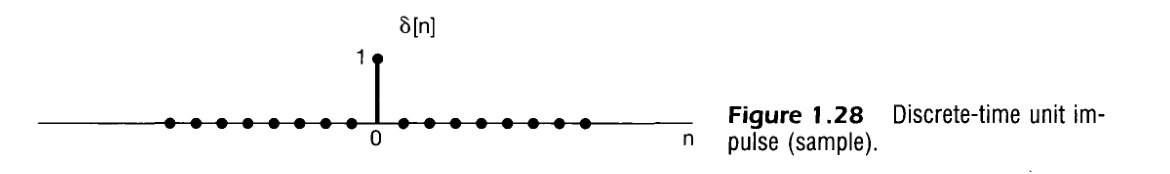
\includegraphics[width=0.8\linewidth]{img/image_2022-09-16-14-12-45.png}
\end{figure}
\end{definition}


Another basic signal is the \textbf{unit step} function, $ u[n] $

\begin{definition}
	
\begin{equation}
	u[n] = \begin{cases}
		0 & n < 0 \\
		1 & n \geq 0
	\end{cases}
\end{equation}
\begin{figure}[H]
	\centering
	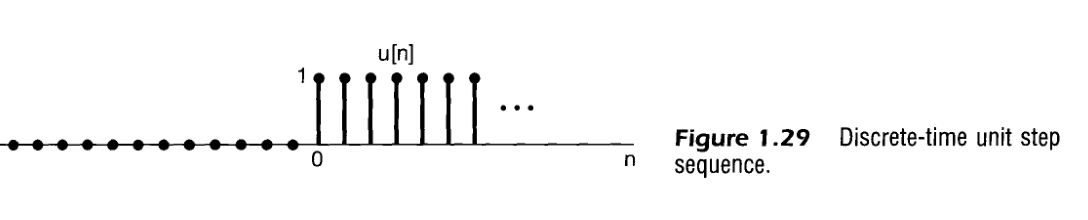
\includegraphics[width=0.8\linewidth]{img/image_2022-09-16-14-13-03.png}
\end{figure}
\end{definition}


The unit impulse function is the first difference of the discrete time step function, i.e.

\begin{equation}
	\delta[n] = u[n] - u[n-1]
\end{equation}

And the unit step function is the running sum of the unit impulse function, i.e.

\begin{equation}
	u[n] = \sum_{m=-\infty}^n \delta[m]
\end{equation}

This can be rewritten with $ k = n-m $ to make a more convenient expression for moving the function along $ -\infty\ldots0\ldots\infty $ 

\begin{equation}
	u[n] = \sum_{k=0}^\infty \delta[n-k]
\end{equation}




\begin{theorem}
	
The unit impulse function $ \delta[n-n_0] $ can be used to sample a function at a specific $ n = n_0 $ since the impulse function will take on the value $ 0 $ for all values of $ n \neq  n_0$ 
\begin{equation}
	x[n] \delta[n-n_0] = x[n_0]\delta[n-n_0]
\end{equation}
\end{theorem}





The continuous equivalents of the unit impulse and unit step functions are defined similarly

\begin{definition}
	
\begin{equation}
	u(t) = \begin{cases}
		0 & t < 0 \\
		1 & t > 0
	\end{cases}
\end{equation}
\end{definition}


Likewise, the continuous unit step function is a running \st{sum} integral of the continuous unit impulse function

\begin{equation}
	u(t) = \int^{t}_{-\infty} \delta(\tau)d\tau
	\label{eq:355:unit_step_cont}
\end{equation}


A relationship analogous to the discrete case can be found for the continuous case; the continuous unit impulse function can be thought of as the first derivative of the continuous-time unit step function

\begin{definition}
\begin{equation}
	\delta(t) = \frac{du(t)}{dt}
	\label{eq:355:unit_impulse_continuous}
\end{equation}
	
\end{definition}


\eqref{eq:355:unit_impulse_continuous} is discontinuous at $ t=0 $ so it is non-differentiable. We can address this by considering an approximation of \eqref{eq:355:unit_impulse_continuous} for a $ \Delta $ short enough to not matter for any practical purpose

\begin{figure}[H]
	\centering
	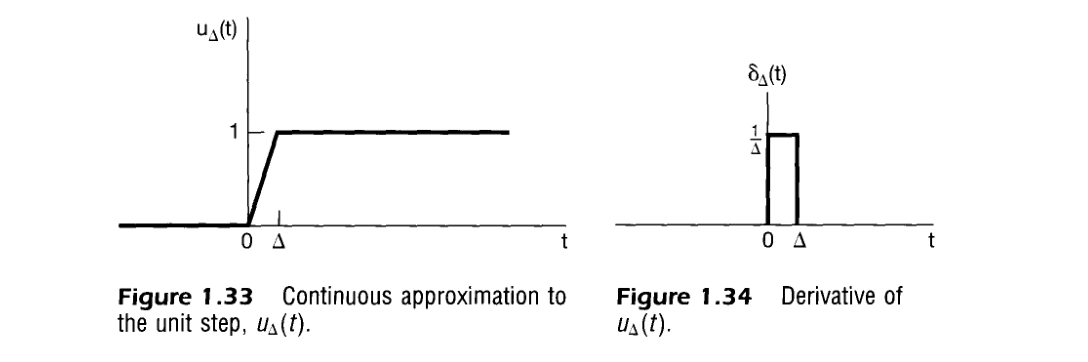
\includegraphics[width=0.8\linewidth]{img/image_2022-09-16-16-53-20.png}
\end{figure}


\eqref{eq:355:unit_step_cont} can be rewritten as follows to make it more convenient to use along $ \sigma\in-\infty\ldots 0\ldots\infty$. 

\begin{equation}
	u(t) = \int^{\infty}_0 \delta(t-\sigma) d\sigma
\end{equation}

\begin{theorem}
	
And by the same argument as for the discrete case, the continuous impulse function has an important sampling property.

	For any arbitrary point $ t_0 $,

	\begin{equation}
		x(t) \delta t(t-t_0) = x(t_0)\delta(t-t_0)
	\end{equation}

\end{theorem}





% 355 END


\part{ECE360: Electronics}

\marginnote{Taught by Prof. Khoman Phang}

\section{Admin and Preliminary}

\subsection{Lecture 1}



\subsubsection{Mark Breakdown}

\begin{table}[H]
	\centering
	\caption{Mark Breakdown}
	\begin{tabular}{|c|c|}
		\hline
		Test 1 & 15 \\
		Test 2 & 20 \\
		Homework & 10 \\
		Labs & 12 \\
		Final & 43 \\
		\hline
	\end{tabular}
\end{table}

\subsubsection{Diodes}

Diodes are an electronic valve which causes current to only flow in one direction.
An ideal diode is an open circuit in the closed direction and a closed circuit in the other, so the current is always in the direction of the arrow (+'ve @ arrow base, -'ve at arrow point)\sn{recall: passive sign convention}.


\begin{figure}[H]
	\centering
	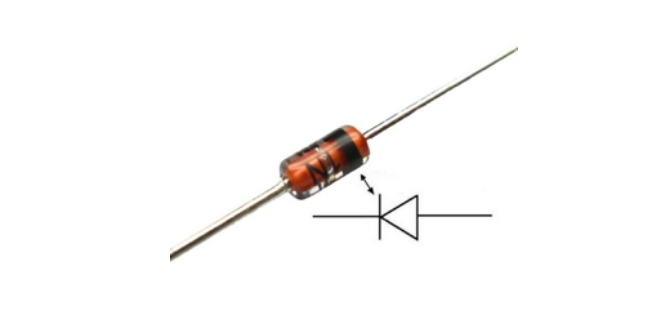
\includegraphics[width=0.8\linewidth]{img/360_diode.png}
	\caption{A diode and its symbol}
	\label{fig:360:diode}
\end{figure}


An example of a diode circuit is the half-wave rectifier which turns an AC signal to a DC signal \marginnote{Can take oscilloscope over resistor to see that a pure DC signal has been generated}

\begin{figure}[H]
	\centering
	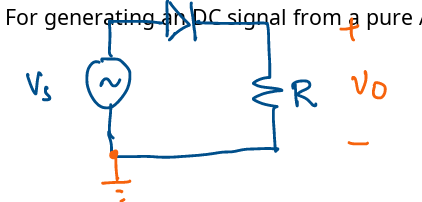
\includegraphics[width=0.8\linewidth]{img/image_2022-09-09-12-51-30.png}
\end{figure}

\begin{figure}[H]
	\centering
	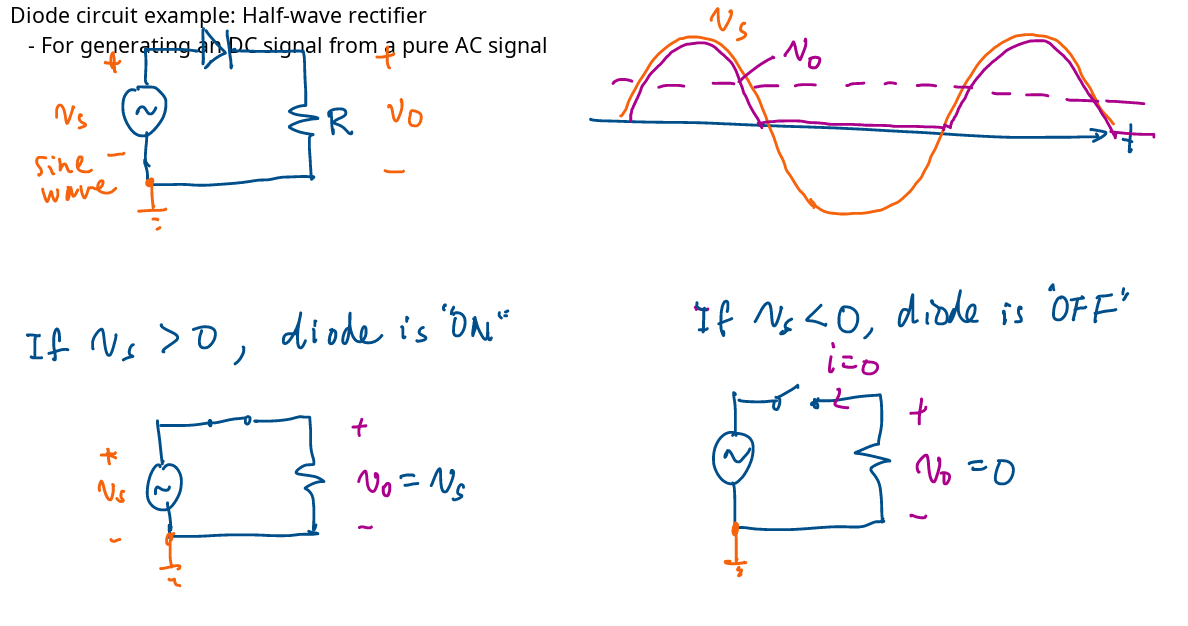
\includegraphics[width=0.8\linewidth]{img/image_2022-09-09-13-01-02.png}
\end{figure}

\section{Diodes}

\subsection{Lecture 2}

More formally, off/on for diodes should be referred to as:
\begin{itemize}
	\item Off $ \leftrightarrow $ reverse bias
	\item On $ \leftrightarrow $ forwards bias
\end{itemize}

\begin{figure}[H]
	\centering
	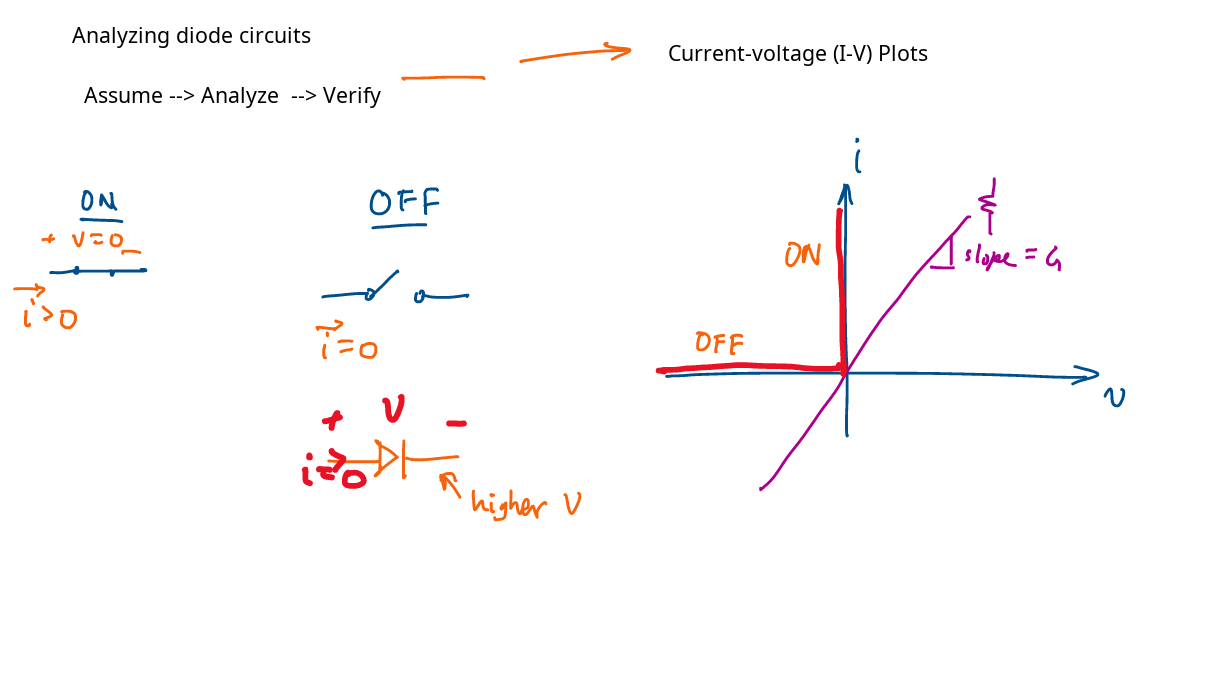
\includegraphics[width=0.8\linewidth]{img/image_2022-09-12-09-41-11.png}
	\caption{General steps for analyzing non-linear circuits. Note plotting out expected response}
\end{figure}





\marginnote{An example of how this is used in circuit design is to manage two power sources. Consider an Arduino that could be powered by an AC adapter or by a computer's USB port. This circuit would choose the higher voltage source and prevent backflow into the other power source due to any potential power differentials. It is also effectively an OR gate}
\begin{figure}[H]
	\centering
	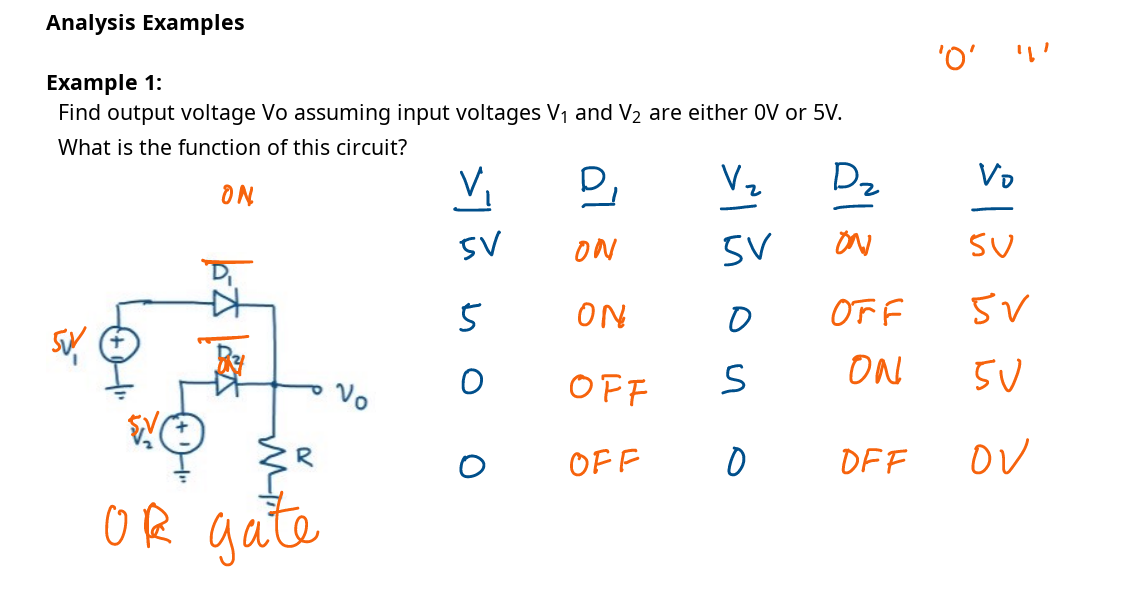
\includegraphics[width=0.8\linewidth]{img/image_2022-09-12-09-54-03.png}
\end{figure}




\begin{figure}[H]
	\centering
	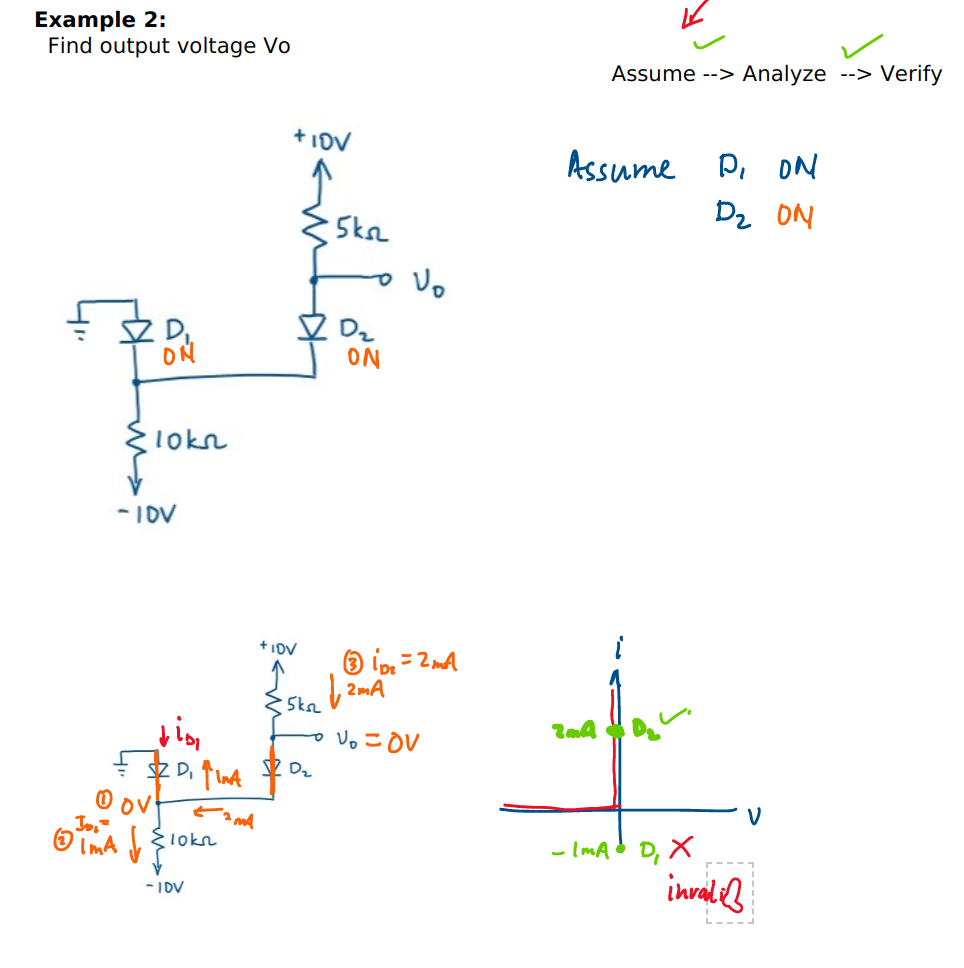
\includegraphics[width=0.8\linewidth]{img/image_2022-09-12-10-02-42.png}
\end{figure}

In this example the initial assumption was incorrect. 

Let's try another analysis with $ D_1  $ off and $ D_2 $ on:

\begin{figure}[H]
	\centering
	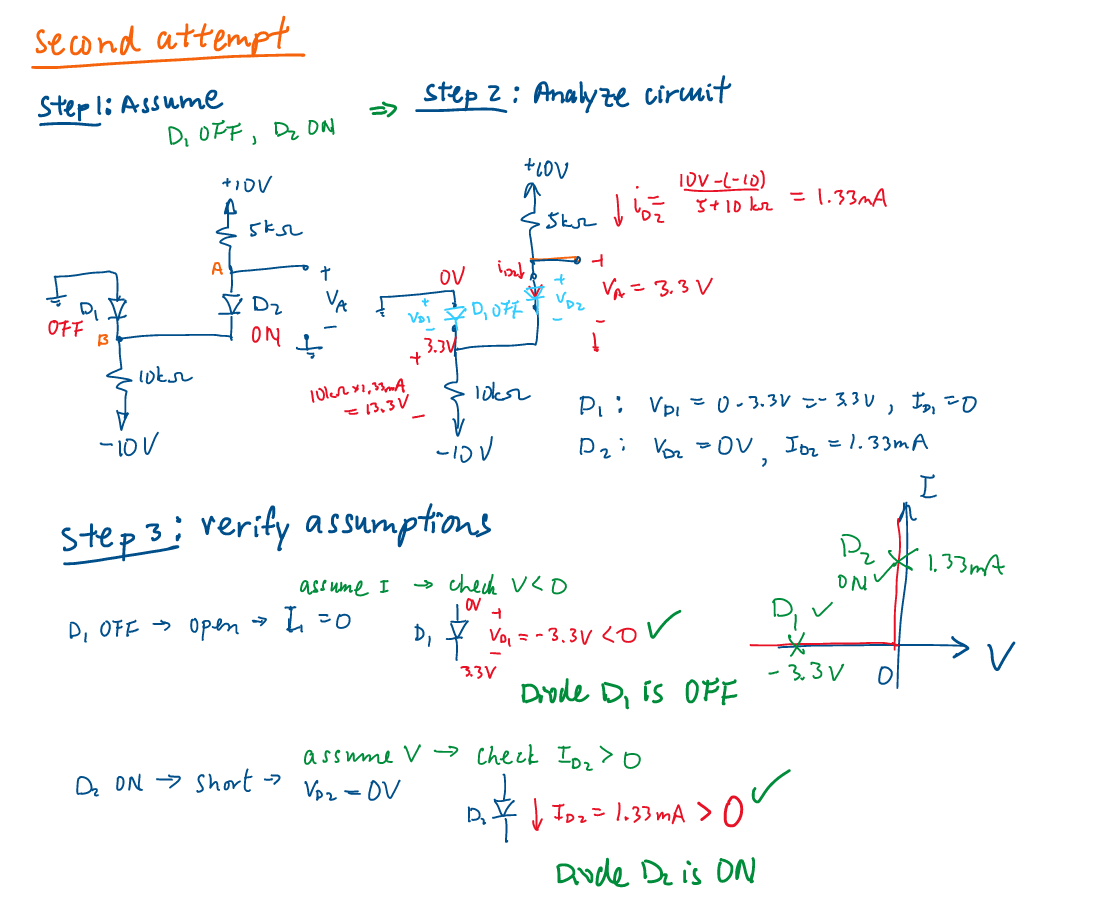
\includegraphics[width=0.8\linewidth]{img/image_2022-09-13-13-20-51.png}
\end{figure}

If we were to do this brute force we'd have to consider 4 cases, so it's important to build up some sort of intuition for the circuit.


\subsection{Lecture 3}


Today we're going to look at the characteristics of real diodes.



\begin{figure}[H]
	\centering
	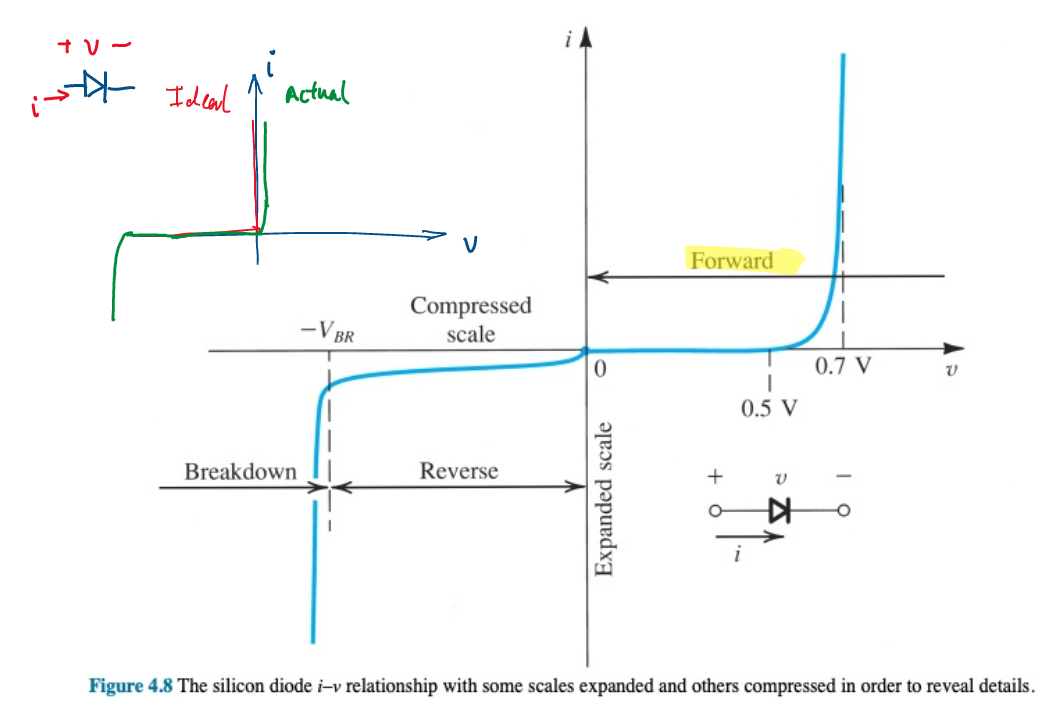
\includegraphics[width=0.8\linewidth]{img/image_2022-09-13-13-26-58.png}
\end{figure}

Real diodes have a little bit of leakage current and also encounter a breakdown point where they're no longer able to block the current.

\begin{theorem}
	\textbf{Forward Bias} 

	\begin{equation}
		i = I_s(e^{\frac{V}{V_T} - 1})
		\label{eq:360:forward_bias}
	\end{equation}

	Where:
	\begin{equation}
		V_T = \frac{kT}{q} \quad [V]
	\end{equation}
	\marginnote{$ k $ is Boltzmann's constant, $ T $ is temperature in Kelvins, $ q $ is the charge of an electron.}

	Most of the time we can assume that the circuit is at room temperature and that $ v_T = 25mV $.
	Note that this value explodes when $ V > V_T  $ which is the breakdown point.
	When encountering a reverse bias $ V_s < 0 $, the $ -1 $ term comes in and causes $ i \approx I_s  $  \marginnote{$ I_s $ is the scale current which is usually $ \approx 1pA $, which doesn't change much until the breakdown point.}

	The scale current is just a general constant which varies in range from $ 10^{-9} to 10^{-15} A $ and scales with temperature, doubling with every approximately $ 5^o C $ increase in temperature.





	Note: the ideal diode equation can be rearranged to find an expression for voltages

	\begin{equation}
		V = V_T \ln{(\frac{i}{I_s}) = \ln{(10)} V_T \log_{10}{(\frac{i}{I_s})}}
		\label{eq:360:forward_bias_v}
	\end{equation}

	These expressions turns out to be quite reliable for reasonable diodes to reasonable voltages.

\end{theorem}

Using the ideal diode equation we can find the relationship between voltages and currents as they pass through the diode.


\begin{equation}
	\frac{i_2}{i_1} = \frac{I_s e^{\frac{V_2}{V_T}}}{I_s e^{\frac{V_1}{V_T}}} = e^{\frac{V_2 - V_1}{V_T}}
\end{equation}


\begin{equation}
	V_2 - V_1 = V_T \ln{(\frac{i_2}{i_1})} \xrightarrow{\text{room temperature}} 60mV \log_{10} \frac{i_2}{i_1}
\end{equation}





\begin{example}
	\begin{figure}[H]
		\centering
		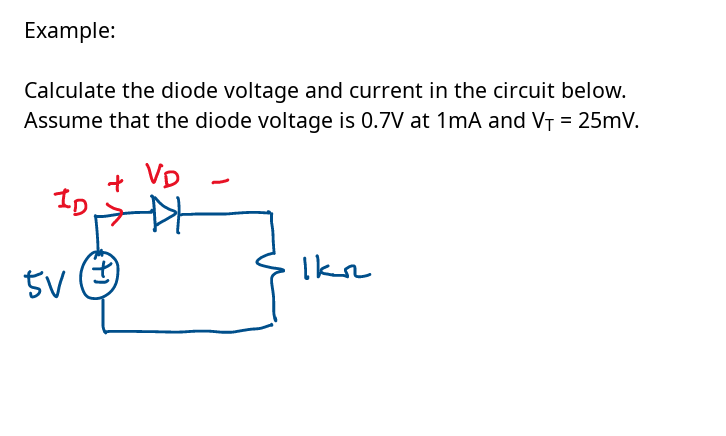
\includegraphics[width=0.8\linewidth]{img/image_2022-09-13-13-55-18.png}
	\end{figure}

	Recall \eqref{eq:360:forward_bias}. Plugging in the given values gives us the scale current.

	\begin{equation}
		1mA = I_s e^{\frac{0.7V}{25mV}}, I_s = 6.9 \cdot 10^{-16} A \Rightarrow I_o = I_s e^{v_o/v_T}
	\end{equation}

	Ohm's law can then be applied at the resistor

	\marginnote{$ V_D $ is the voltage across the diode }

	\begin{equation}
		V_r = IR = I_oR  = 5V - V_D \Rightarrow 5 - V_D = I_o R
	\end{equation}

	So we have two equations and two unknowns (since we know $ v_T = 25mV $ but $ v_o $ was used at first just to find $ I_s $ ) Solving for the unknowns gives us:

	\begin{itemize}
		\item $ V_o  = 0.736 V $
		\item $ I_D = 4.264 mA $ 
	\end{itemize}
\end{example}


\section{Lecture 4: Forward conducting diodes}


The exponential model accurately describes the diode outside of the breakdown region, though it's nonlinear behaviour makes it difficult to use.

For $ V_{DD} > 0.5V $ \marginnote{$ V_{DD} $ denotes a DC power supply}

\begin{equation}
	I_D = I_S e^{V_D/V_T}
	\label{eq:360:forward_conducting_diode}
\end{equation}

Where 
\begin{itemize}
	\item $ I_S $ is the diode parameter
	\item $ V_T $ is the thermal voltage
\end{itemize}

Another equation may be produced via Kirchhoff's law

\begin{equation}
I_D = \frac{V_{DD} - V_D}{R}
 \label{eq:360:forward_conducting_diode_kirchhoff}
\end{equation}



The unknown quantities $ I_D $ and $ V_D $ may be solved for via graphical analysis or iteration.

\begin{example}

	This simple circuit is used to demonstrate the exponential model of the diode.
	\begin{figure}[H]
		\centering
		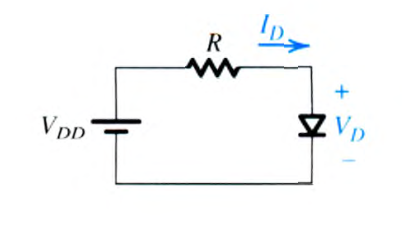
\includegraphics[width=0.8\linewidth]{img/image_2022-09-16-22-33-11.png}
		\caption{Simple example circuit with diode}
		\label{fig:360:forward_conducting_diode_example}
	\end{figure}
	
	Plots of the diode characteristics and Kirchhoff's relation are plotted, the intersection of which gives the solution.

	\begin{figure}[H]
		\centering
		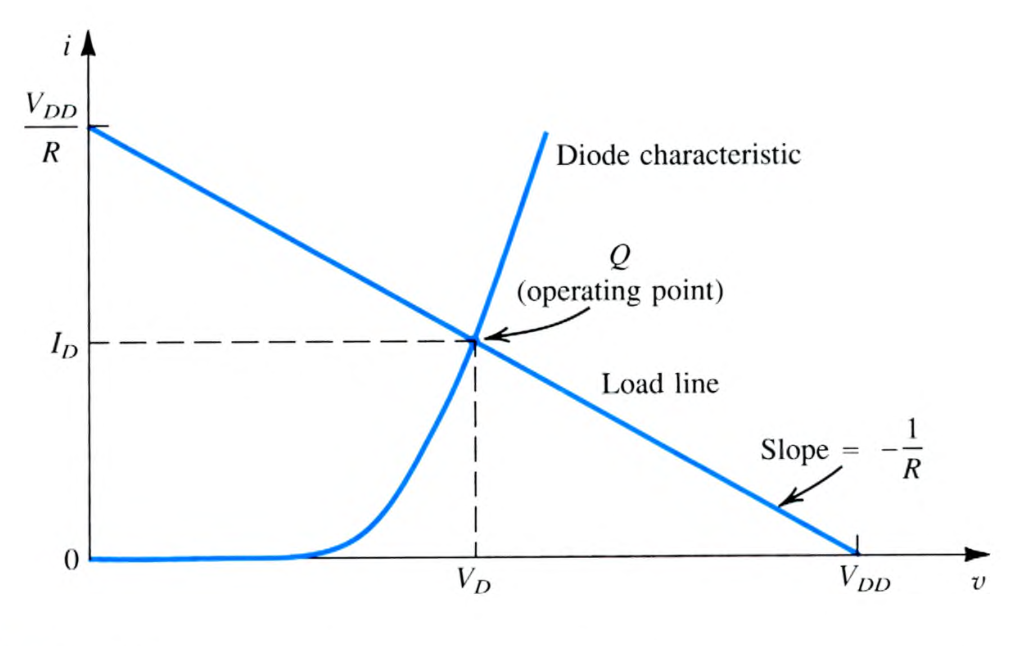
\includegraphics[width=0.8\linewidth]{img/image_2022-09-16-22-32-51.png}
	\end{figure}
\end{example}

An iterative procedure may also be applied to solve for the unknowns, the procedure for which will be illustrated through an example


\begin{example}

	Find $ I_D, V_D $ for the circuit in the previous example (Fig.~\ref{fig:360:forward_conducting_diode_example}). $ V_{DD} = 5V, R = 1k\Omega $, and at $ V_{D} 0.7V, I_D = 1mA $ 


\begin{enumerate}
	\item Assume $ V_D = 0.7V$, then use \eqref{eq:360:forward_conducting_diode_kirchhoff} to find $ I_D $.
		\begin{equation}
			I_D = \frac{5V - 0.7V}{1k\Omega} = 4.3mA
		\end{equation}
		
	\item Use the diode equation \eqref{eq:360:forward_conducting_diode} to get a better estimate for $ V_D $.

		\begin{equation}
			V_2 - V_1 = 2.3 V_T \log \frac{I_2}{I_1} \Rightarrow V_2 = V_1 + 0.06 \log \frac{I_2}{I_1}
		\end{equation}
	substituting $ V_1 = 0.7V, I_1 = 1mA, I_2 = 4.3mA $,
	\begin{equation}
		V_2 = 0.738V \Rightarrow I_D = 4.3mA, V_D = 0.738V
	\end{equation}
	\begin{itemize}
		\item This states that for a decade\mn{Factor of 10} change in current the diode voltage drop changes by $ 2.3(V_T \approx 60mV) $ which is negligibly small for $ v < 0.5V $. 
		The voltage at which the this behaviour becomes significant is called the \textbf{cut-in voltage} 
	\end{itemize}

\item Repeat steps 1 and 2 with the new values until the values more or less become stable
\end{enumerate}
\end{example}

This iterative model is powerful and yields accurate results, but can be computationally expensive especially when calculating by hand.
To address this we employ other models such as the \textit{constant-voltage-drop} model which approximates the exponential characteristics via a piecewise linear model.
The reason why this is possible is because forward conducting diodes exhibit a voltage drop that varies in a relatively narrow range.

\begin{figure}[H]
	\centering
	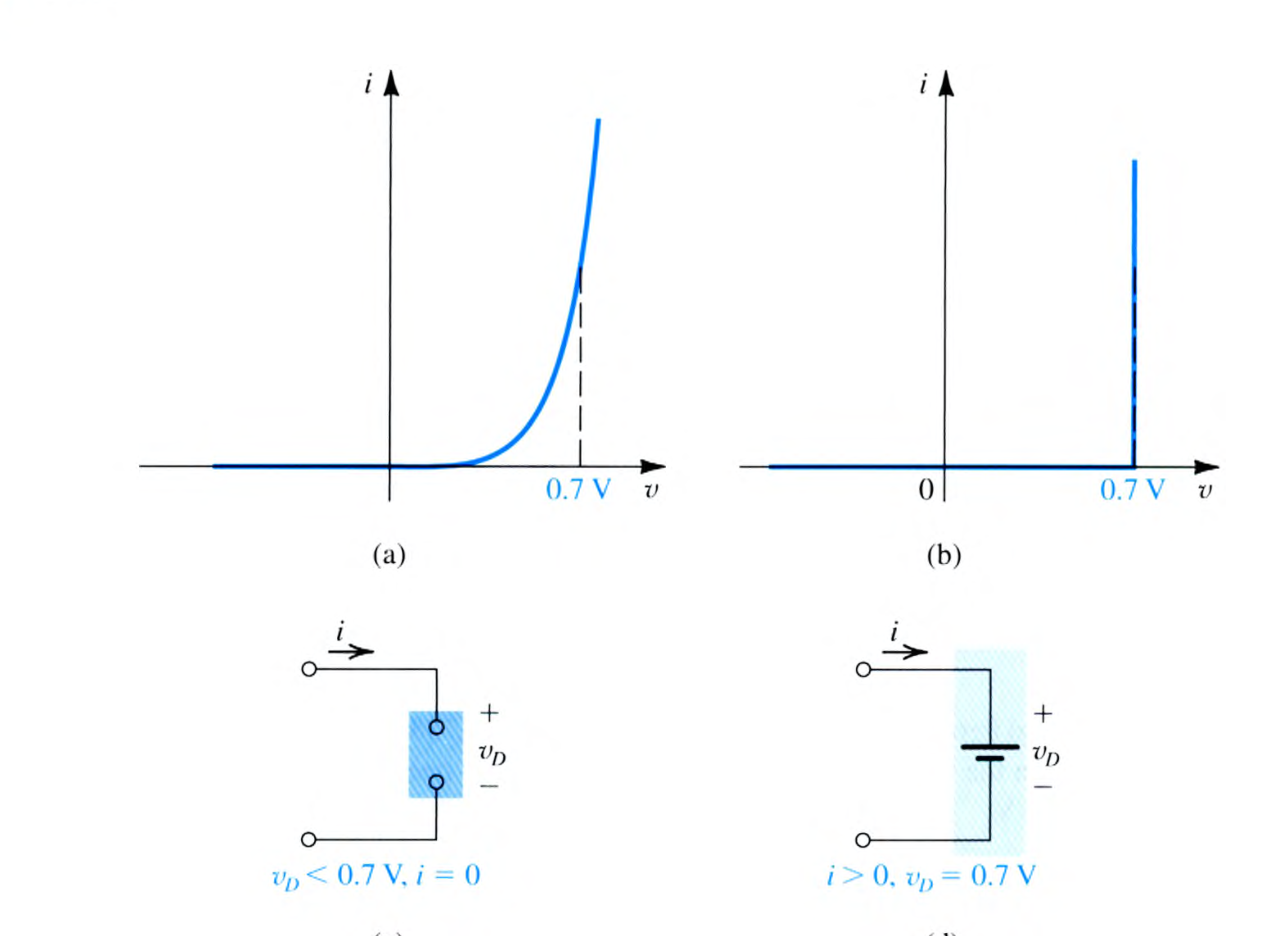
\includegraphics[width=0.8\linewidth]{img/image_2022-09-16-22-49-19.png}
\end{figure}


Using the constant voltage drop model in our analysis looks the same as before, but with $ V_D $ directly taking on the value of $ 0.7V $ (as per the prior example) instead of being solved for with the diode equation.



In applications that involve voltages greater than the voltage drop (i.e. usually $ \approx 0.6-0.8V $  ) we can neglect the diode voltage drop altogether while calculating the diode current.

\begin{equation}
	\begin{split}
		V_D &= 0V \\
		 I_D &= \frac{5-0}{1} = 5mA  \\
	\end{split}
	\label{eq:}
\end{equation}



This is generally good enough for a first estimate, though the previous model isn't that much more work and gives more accurate results.
The primary use of this model is to determine which diodes are on or off in a multi-diode circuit


\subsubsection{Small-Signal Model}


The small signal method is an alternative model used to describe the nonlinear diode's characteristics with greater accuracy than piecewise linear models\marginnote{Similar methods will be applied to transistors in later chapters}.


Consider a small $ \Delta V_{DD} $ applied to the diode, which would cause a small $ \Delta I_D, \Delta V_D $.
We want to find a quick way of determining the values of these incremental changes.

\begin{figure}[H]
	\centering
	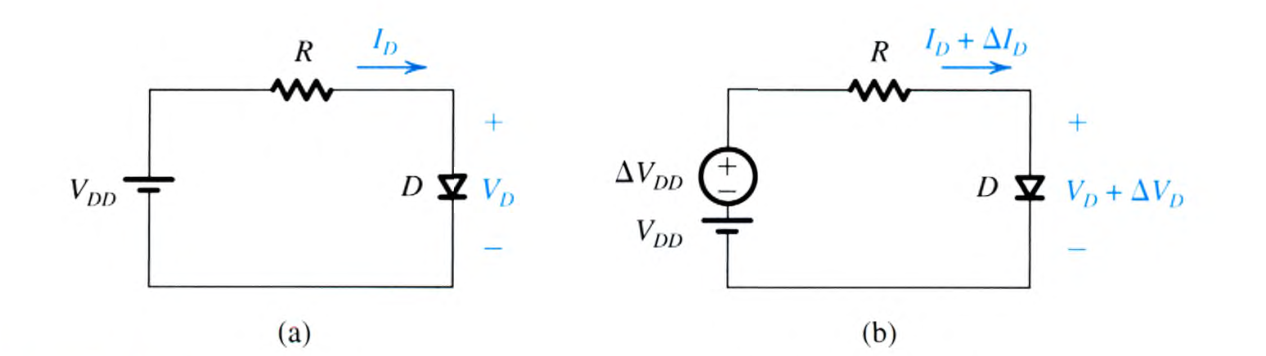
\includegraphics[width=0.8\linewidth]{img/image_2022-09-16-23-15-07.png}
\end{figure}

Skipping a bunch of math\sidenote{It is 11:17pm and I have two more lectures to catch up to today} the results are as follows:


\begin{definition}

	\textbf{Small signal approximation} 
	\begin{equation}
		i_D(t) \approx I_D (1+ \frac{v_d}{V_T} )
	\end{equation}
	This is valid for when variations in diode voltage $ |v_d| \lessapprox 5mV$ 


	The quantity relating $ i_d $ to $ v_d $  is the diode small-signal resistance


	\begin{equation}
	 r_d = \frac{V_T}{I_D} 
	 \label{eq:360:small_signal_diode_resistance}
	\end{equation}
	
\end{definition}


\marginnote{Small signal analysis can be performed separately from the dc bias analysis because of the linearization of diode characteristics in the small-signal approximation}

The steps for calculating the small signal model are as follows:

\begin{enumerate}
	\item Perform a dc analysis using the exponential, constant-voltage-drop, or piecewise-linear model.
	\item Linearise the circuit. For a forward-based diode, find $ r_d $ by substitution $ I_D $   into \eqref{eq:360:small_signal_diode_resistance}. The small-signal equivalent circuit is found by eliminated all independent dc sources\sidenote{since we already accounted for them in step 1} and replacing the diode with its small-signal resistance $ r_d $ 
	\item Solve the linearised circuit. In particular we would want to find $ \Delta I_D, \Delta V_D $ and check to see if it is consistent with our approximation, i.e. that $ \Delta V_D \lessapprox 5mV $ 
\end{enumerate}




% 360 END







\part{ECE358: Foundations of Computing}

\marginnote{Taught by Prof. Shurui Zhou}

\section{Admin and Preliminary}

\subsection{Lecture 1}

Topics covered will include:
\begin{itemize}
	\item Graphs, trees
	\item Bunch of sorts
	\item Fancy search trees; red-black, splay, etc
	\item DP, Greedy
	\item Min span tree, single source shortest paths
	\item Maximum flow
	\item NP Completeness, theory of computation
	\item Blockchains??
	\item $ \Theta $ 
\end{itemize}

Solutions will be posted on the window of SF2001. Walk there and take a picture.

\subsubsection{Mark Breakdown}

\begin{table}[H]
	\centering
	\caption{Mark Breakdown}
	\begin{tabular}{|c|c|}
		\hline
		Homework x 5 & 25 \\
		Midterm (Open book) & 35 \\
		Final (Open book) & 40\\
		\hline
	\end{tabular}
\end{table}



\section{Complexities}


\subsection{Lecture 2}


This lecture we talked about big O notation. For notes on this refer to my tutorial notes for ESC180, ESC190: \href{https://github.com/ihasdapie/teaching/}{https://github.com/ihasdapie/teaching/}


\begin{definition}
	Big O notation (upper bound)

	$ g(n) $  is an asymptotic upper bound for $ f(n) $ if:

	\begin{equation}
		O(g(n)) = \left\{f(n): \exists \quad c, n_0 \quad s.t. \quad 0 \le  f(n) \le  c\cdot g(n), \forall n \ge  n_o \right\}
		\label{eq:358:bigOh}
	\end{equation}
\end{definition}

\begin{proof}

	\textbf{What is the big-O of $ n! $ }?
	\begin{equation}
			n! \le n \cdot n \cdot n \cdot  n \ldots n = n^n \Rightarrow n! \in O(n^n) 
	\end{equation}
\end{proof}



\begin{definition}
	Big $ \Omega $  notation (lower bound)

	$ h(n) $  is an asymptotic lower bound for $ f(n) $ if:
	\begin{equation}
		\Omega(h(n)) =  \left\{f(n): \exists \quad {c, n_0} > 0 \quad s.t. \quad 0 \le c \cdot h(n) \le  f(n), \forall n \ge  n_o \right\}
		\label{eq:358:bigOmega}
	\end{equation}
\end{definition}

\begin{proof}

	\textbf{Find $ \Theta $ for $ f(n) \sum^n_i i $}.

	For this we will employ a technique for the proof where we take the right half of the function, i.e. from $ \frac{n}{2} \ldots n $ and then find the bound

	\begin{equation}
		\begin{split}
			f(n) &= 1 + 2 + 3 \ldots + n \\
			 &\ge \lceil \frac{n}{2} \rceil + (\left\lceil \frac{n}{2} \right\rceil + 1) + (\left\lceil \frac{n}{2} \right\rceil + 2) + \ldots n \quad \text{$ n/2 $ times} \\
			 &\ge \left\lceil \frac{n}{2} \right\rceil +   \left\lceil \frac{n}{2} \right\rceil + \left\lceil \frac{n}{2} \right\rceil +  \ldots \left\lceil \frac{n}{2} \right\rceil \\
			 &\ge \frac{n}{2} \cdot \frac{n}{2} \\
			 &= \frac{n^2}{4} \\
		\end{split}
	\end{equation}

	And therefore for $ c = \frac{1}{4} $  and $ n = 1 $ , $ f(n) \in \Theta(n^2) $ 
	
	
\end{proof}



\begin{definition}
	Big $ \Theta $  notation (asymptotically tight bound)

	\begin{equation}
		\Theta(g(n)) = \left\{ f(n) : \exists \quad c_1 c_2, n_0 \quad s.t. \quad 0 \le  c_1 g(n) \le  f(n) \le  c_2 g(n), \forall n \ge  n_o   \right\}
		\label{eq:358:bigTheta}
	\end{equation}
\end{definition}

\begin{proof}
	Prove that 

	\begin{equation}
		\sum^n_{j=1} i^k = \Theta(n^{k+1})
	\end{equation}

	First, prove $ O(f(n)) = O(n^{k+1}) $ 

	\begin{equation}
		\begin{split}
			f(n) = \sum^n_{j=1} i^k &= 1^k + 2^k + \ldots n^k \\
			 &\le n^k + n^k + \ldots n^k  \\
			 &= n^{k+1} \\
		\end{split}
	\end{equation}


	Next, prove $ \Omega(f(n)) = \Omega(n^{k+1}) $ 

	\begin{equation}
		\begin{split}
			f(n) = \sum^n_{j=1} i^k &= 1^k + 2^k + \ldots n^k \\
			 &= n^k + (n_1)^k + \ldots 2^k + 1^k = \sum^n_{i=1} (n-i+1)^k \\
			 &\ge   \frac{n}{2}^k * n \ge \frac{n^{k+1}}{2^k} = \Omega(n^{k+1}) \\
		\end{split}
	\end{equation}

	Therefore $ f(n) = \Theta(n^{k+1}) $ 
\end{proof}

Note that we may not always find both a tight upper and lower bound so not all functions have a tight asymptotic bound.







\begin{theorem}
	\textbf{Properties of asymptotes:} 

	Note: $\land $ means AND

	\textbf{Transitivity} \mn{The following applies to $ O, \Theta, o, \omega $ }
	\begin{equation}
		(f(n) = \Theta(g(n)) \land g(n) = \Theta(h(n))) \Rightarrow f(n) = \Theta(h(n))
		\label{eq:358:asymptotic_transitivity}
	\end{equation} 


	\textbf{Reflexivity}\mn{The following applies to $ O, \Theta $ }
	\begin{equation}
		f(n) = \Theta(f(n))
		\label{eq:358:asymptotic_reflexivity}
	\end{equation}
	
	\textbf{Symmetry}
	\begin{equation}
		f(n) = \Theta(g(n)) \iff g(n) = \Theta(f(n))
		\label{eq:358:asymptotic_symmetry}
	\end{equation}
	

	\textbf{Transpose Symmetry}

	\begin{equation}
		\begin{split}
			 f(n) &= O(g(n)) \iff g(n) = \Omega(f(n))  \\
			 f(n) &= o(g(n)) \iff g(n) = \omega(f(n))  \\
		\end{split}
		\label{eq:358:asymptotic_transpose_symmetry}
	\end{equation}

\end{theorem}


Runtime complexity bounds can sometimes be used to compare functions. For example, $ f(n) = O(g(n)) $ is like $ a \le b $

\begin{itemize}
	\item $ O \approx \le $
	\item $ \Omega \approx \ge  $ 
	\item $ \Theta \approx \approx  $ 
	\item $ o \approx < $; an upper bound that is \textbf{not}  asymptotically tight
	\item $ \omega > $ a lower bound that is \textbf{not}  asymptotically tight
\end{itemize}

Note that there is no trichotomy; unlike real numbers where we can just do $ a<b $, etc, we may not always be able to compare functions.

\begin{figure}[H]
	\centering
	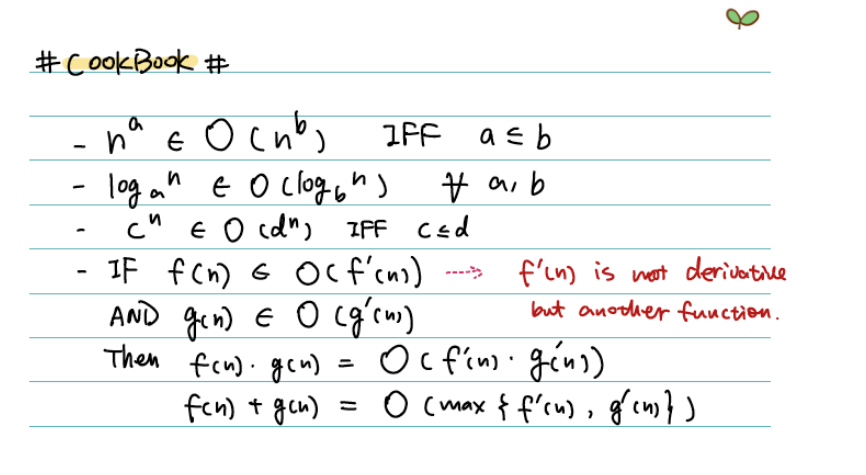
\includegraphics[width=0.8\linewidth]{img/image_2022-09-13-00-26-01.png}
	\caption{Complexity Cookbook}
	\label{fig:358:complexity_cookbook}
\end{figure}

\subsection{Lecture 3: Logs \& Sums}

\marginnote{
	Recall:
	\begin{equation}
		a = b^c \Leftrightarrow log_ba = c
	\end{equation}
}


\subsubsection{Functional Iteration}

$ f^{(i)}(n) $  denotes a function iteratively applied $ i $ times to value $ n $.

For example, a function may be defined as:
\begin{equation}
	f^{(i)}(n) = 
	\begin{cases}
		f(n) & \text{if } i = 0 \\
		f(f^{(i-1)}(n)) & \text{if } i > 0
	\end{cases}
	\label{eq:358:functional_iteration_1}
\end{equation}


Given \eqref{eq:358:functional_iteration_1} we see that 

\begin{enumerate}
	\item $ f(n) = 2n $ 
	\item $ f^{(2)}(n) = f(2n) = 2^2n$ 
	\item $ f^{(3}(n) = f(f^{(2)}(n)) = 2^3n$ 
	\vdots
	\item $ f^{(i)}(n) = 2^in $
\end{enumerate}


As an exercise we may look at an iterated logarithm function, 'log star`

\begin{equation}
	lg^*(n) = \min\{ i \ge  0 : lg^{(i)} n \le  1 \}
	\label{eq:358:iterated_logarithm}
\end{equation}

This describes the number of times we can iterate $ log(n) $ until it gets to $ 1 $ or smaller.

\begin{itemize}
	\item $ log^*2 = 1 $ 
	\item $ log^*4 = 2 = log^*2^2 = 1 + log^*2 = 2 $ 
		\vdots
	\item for practical reasons $ log^* $  doesn't really get bigger than $ 5 $. This is one of the slowest growing functions around.
\end{itemize}


\textbf{Summations \& Series} 

\begin{proof}

	Proof for a finite geometric sum:

	\begin{equation}
		\begin{split}
			\sum^n_{k=0} x^k &= S \\
			 S &= 1 + x + x^2 \ldots x^n  \\
			 xS &= x + x^2 + x^3 \ldots x^{n+1} \\
			 S &= \frac{1-x^{n+1}}{1-x} \\
		\end{split}
	\end{equation}
\end{proof}


\begin{equation}
	\sum^\infty_{i=1} x^i = \frac{1}{1-x} \quad \text{if } |x| < 1
	\label{eq:358:decreasing_geometric_series}
\end{equation}

\begin{equation}
	\sum^\infty_{k=0} kx^k = \frac{x}{(1-x)^2} \quad \text{if } |x| < 1
	\label{eq:358:geometric_series_2}
\end{equation}

\begin{proof}

	Begin by differentiating both sides over $ x $ 

	\begin{equation}
		\sum^\infty_{k=0} x^k = \frac{1}{(1-x)} \quad \text{if } |x| < 1
	\end{equation}

	\begin{equation}
		\sum^{\infty}_{k=0} kx^{k-1} = \frac{1}{(1-x)^2}
	\end{equation}

	And then multiply both sides by $ x $, therefore \eqref{eq:358:geometric_series_2} follows.
\end{proof}

\textbf{Telescoping Series} 

\begin{equation}
	\sum_{k=1}^{n} a_k - a_{k-1} = a_n - a_0
\end{equation}

\begin{proof}
	Write it out and cancel out terms
	\begin{equation}
		(a_1 - a_0) + (a_2 - a_1) \ldots (a_n - a_{n-1}) = a_n - a_0
	\end{equation}
	Therefore the sum telescopes
\end{proof}


Another telescoping series may be proved similarly:
\begin{equation}
	\sum^{n-1}_{k=1} \frac{1}{k(k+1)} \xrightarrow{math} \sum^{n-1}_{k=1} (\frac{1}{k} - \frac{1}{k+1}) 
	= 
	(1- \frac{1}{2}) + \ldots (\frac{1}{n-1} - \frac{1}{n}) = a_o - a_n
\end{equation}


\subsection{Lecture 4: Induction \& Contradiction}

% 358 END



\part{MAT389: Complex Analysis}

\marginnote{Taught by Prof. Sigil}
\section{Complex Numbers}
\subsection{Lecture 1}

Consider a 2-vector $ \vec{x} = (x, y) \in \mathcal{R} $. 
As complex numbers correspond to two-vectors 

\begin{equation}
	\vec{x} = (x, y) \leftrightarrow z = x + iy, i^2 = -1
\end{equation}

$ z $ is, therefore, a complex variable. What are the benefits of a complex number like $ z $?


\marginnote{This prof lectures at the speed of sound and talks \textit{into} the board. Couldn't quite follow during this lecture, hopefully I get better about it in the following ones.}
\begin{definition}

	\textbf{Imaginary and Complex Numbers} 

	$ i $ is an imaginary number such that
	\begin{equation}
		i^2 = -1
		\label{eq:389:i}
	\end{equation}

	A complex number has the form:
	\begin{equation}
		z = x + iy
		\label{eq:389:complex}
	\end{equation}
\end{definition}

\begin{definition}

	There are a number of operations we can perform on complex numbers.

	\textbf{Addition} 

	\begin{equation}
		z + z^\prime = (x + x^\prime) + i(y + y^\prime)
		\label{eq:389:complex_add}
	\end{equation}


	\textbf{Multiplication} 
	\begin{equation}
		z z^\prime = (x + iy)(x^\prime + iy^\prime) = (x x^\prime - y y^\prime) + i(x y^\prime + x^\prime y)
		\label{eq:389:complex_mult}
	\end{equation}


	\begin{proof}
		Proof of \eqref{eq:389:complex_mult}:

		\begin{equation}
			\begin{split}
				zz^\prime &= (x+iy)(x^\prime + iy^\prime) \\
				 &= x + ixy^\prime + i yx^\prime + i^2yy^\prime\\
				 &= x x^\prime  - yy^\prime + i(xy^\prime + y x ^\prime) \\
			\end{split}
		\end{equation}
	\end{proof}


	\textbf{Magnitude} 

	\begin{equation}
		|z| = \sqrt{x^2 + y^2}
		\label{eq:389:complex_mag}
	\end{equation}

	\textbf{Conjugate}

	The complex conjugate has the properties:

	\begin{itemize}
		\item $ \overline{z} z = |z|^2 $ 
		\item $ \overline{(z + z^\prime)} = \overline{z} + \overline{z}^\prime$ 
		\item $ \overline{z \cdot z^\prime} = \overline{z} \cdot \overline{z}^\prime $ 
	\end{itemize}


	We can define a new operation

	\begin{equation}
		\forall \text{complex} z, \exists \quad \text{complementary number } w \text{ such that } zw = wz = 1
	\end{equation}

	Denote 

	\begin{equation}
		w = \frac{1}{z} = z^{-1}
		\label{eq:389:complex_inv}
	\end{equation}

	\begin{proof}
		Proof of \eqref{eq:389:complex_inv}:
		Find $ w $ s.t. $ zw = 1 $ 

		\begin{equation}
			\begin{split}
				zw &=1  \\
				 w \overline{z} z&= \overline{z}z = |z|^2 > 0  \\
				 |z|^2 w &= \overline{z}  \\
				 w &= \frac{\overline{z}}{|z|^2} \rightarrow Z^{-1} = \frac{\overline{z}}{|z|^2}\\
			\end{split}
		\end{equation}
		
	\end{proof}

\end{definition}

Furthermore, there are operators that we can define on complex numbers.

\begin{definition}
	\textbf{Real and Imaginary Operators}

	Given $ z = x + iy $, we can define the real and imaginary operators
	\begin{equation}
		x = Re \left\{ z \right\}
	\end{equation}

	\begin{equation}
		y = Im \left\{ z \right\}
	\end{equation}

	\begin{example}
		\begin{equation}
			Im \left\{ (1 = \sqrt{2} i)^-1 \right\} 
		\end{equation}

		By \eqref{eq:389:complex_inv}, we have  


		\begin{equation}
			Im \left\{ z^{-1} \right\} = \frac{-Im \left\{ z \right\} }{|z|^2} 
			\label{eq:389:complex_inv_im}
		\end{equation}

		And

		\begin{equation}
			Re \left\{ z^{-1} \right\} = \frac{-Re \left\{ z \right\} }{|z|^2} 
			\label{eq:389:complex_inv_re}
		\end{equation}

		Using these, for example, we find that the $ Im = \frac{-\sqrt{2} }{3} $

		We can get the real component in a similar way.
		
	\end{example}

\end{definition}


Here is an enumeration of absolute value properties for complex numbers:

\begin{equation}
	| z \cdot  w| = |z| |w|
\end{equation}

\begin{equation}
	|z + w| \le  |z| + |w|
\end{equation}

\begin{equation}
	|\overline{z}| = |z|
\end{equation}

\begin{equation}
	|z + w|^2 = (\overline{x} + \overline{w}) (z + w) = |z|^2 + |w|^2 + \overline{z}w + \overline{w}z
	\label{eq:389:z_plus_w_abs_squared}
\end{equation}

\begin{proof}

Note that $ \overline{z}w + \overline{w}z = 2 Re \left\{ z \overline{w} \right\}  $, by \eqref{eq:389:z_plus_w_abs_squared}

And so 

\begin{equation}
	|z + w|^2 \le  |z|^2 + |w|^2 + 2 |z| |w| = (|z| + |w|)^2
\end{equation}
	
\end{proof}

\subsection{Lecture 2}

Whereas a two-vector $ \vec{x} \in \mathbb{Z} $, complex numbers exist in the complex plane, $ z \in \mathbb{C} $ 

% 389 END


\begin{theorem}
	\textbf{Polar Decomposition} 

	Complex numbers can be expressed in polar form as well
	\begin{equation}
		z = r(cos \theta + i sin \theta)
		\label{eq:389:complex_polar}
	\end{equation}

	Where
	\begin{equation}
		r = |z| \qquad x = rcos \theta \qquad y = rsin \theta
	\end{equation}
\end{theorem}


This has a number of useful properties


\begin{equation}
	z \cdot  z^\prime = |z| |z^\prime| (\cos(\theta + \theta^\prime) + i \sin(\theta + \theta^\prime))
	\label{eq:389:complex_mult_2}
\end{equation}

\begin{equation}
	\frac{z}{z^\prime} = \frac{|z|}{|z^\prime|} (\cos(\theta - \theta^\prime) + i \sin(\theta - \theta^\prime))
	\label{eq:389:complex_div_2}
\end{equation}


\begin{proof}
	Proof for \eqref{eq:389:complex_mult_2}:

	\begin{equation}
		\begin{split}
			z \cdot  z^\prime &= |z|(\cos(\theta + i \sin \theta)) \times |z^\prime| (\cos \theta^\prime + i \sin \theta ^\prime) \\
			 &= |z| |z^\prime| (\cos\theta \cos\theta^\prime + i \cos\theta \sin\theta^\prime + i \sin \theta \cos \theta^\prime - \sin\theta \sin\theta^\prime ) \\ 
			 &= |z| |z^\prime| \left[ \cos\theta \cos \theta^\prime - \sin \theta \sin \theta^\prime   + i (\cos\theta \sin\theta^\prime + \sin\theta \cos\theta^\prime)\right]  \\
		\end{split}
	\end{equation}
	And the proof follows
\end{proof}


\begin{lemma}
	A corollary exists

	\begin{equation}
		z^2 = |z|^2 (\cos2\theta + i \sin 2 \theta)
	\end{equation}
	
\end{lemma}

\begin{theorem}
	\textbf{Moivre's Theorem} 


	\begin{equation}
		z^n = |z|^n (\cos(n\theta) + i \sin(n\theta))
		\label{eq:389:moivre}
	\end{equation}

	So we may define $ z $ to be the $ n^{th} $ root of $ w $ which implies that 

	\begin{lemma}
		Every complex number has a $ n^{th} $ root $ \forall n $ 
	\end{lemma}

	\begin{proof}

		\marginnote{
			Intuition: define $ z $ to be $ \frac{1}{n} $ and then take the $ n^{th} $ power of both sides to show that $ z^n = w $ 
		}
		\begin{equation}
			\text{Let } z = |w|^{\frac{1}{n}}(\cos \frac{\theta}{n} + i \sin \frac{\theta}{n})
		\end{equation}

		Then

		\begin{equation}
			w = |w| (\cos \theta + i \sin \theta), \text{ then  } z^n = w
		\end{equation}
		
	\end{proof}
	
\end{theorem}

This leads us to the conclusion that representations of complex numbers are not unique\sn{They are part of a cyclic group}.
\begin{proof}
	If every $ z $ can be written as $ z = r(\cos\theta + i \sin \theta)$, then it holds for $ \theta + 2\pi n \forall n \in \mathbb{Z} $ since $ \sin\theta = \sin(\theta + 2\pi n) $  and  $  \cos\theta = \cos(\theta + 2\pi n)  $.
\end{proof}

\subsubsection{Functions on complex planes}


\begin{definition}
	Given a domain $ \mathbb{D} \in \mathbb{C} $, a function $ f $  is a rule such that

	\begin{equation}
		z \in \mathbb{D} \xrightarrow{f} w \in \mathbb{D} \leftrightarrow w = f(z)
	\end{equation}
\end{definition}


\begin{definition}
		We may define $ \mathbb{D} $ to be the domain of $ f $ 


		Likewise, range is defined as
			\begin{equation}
				Ran\{f\} = \{ w \in \mathbb{C} : \exists z \in D : f(z) = w \}
			\end{equation}
			
\end{definition}

\begin{example}
	\begin{equation}
		f(z) = \frac{1}{z+i}
	\end{equation}

	What is the maximum domain of $ f $?

	\begin{equation}
		Dom\{f\} = \{ z \in \mathbb{C} : |z| < -i \}
	\end{equation}

	What is the range of $ f $?
	\begin{equation}
		\frac{1}{z+i} = w
	\end{equation}

	For which values of $ w $ can we solve this equation?

	\begin{equation}
		z = -i + \frac{1}{w}
	\end{equation}

	So the range of the function is 
	\begin{equation}
		Ran\{f\} = \{ w \in \mathbb{C} : |w| \neq 0 \}
	\end{equation}
	
	
\end{example}


\begin{example}
	\begin{equation}
		f(z) = z^2 + 1
	\end{equation}

	It is fairly clear that $ Dom\{f\} = {f \in \mathbb{C}} $ 

	The range can be found by solving for $ z $ in

	\begin{equation}
		z^2 + 1 = w
	\end{equation}

	And so 


	\begin{equation}
		Ran\{f\} = \{ w \in \mathbb{C}\}
	\end{equation}
	
	
	
	
\end{example}


\subsubsection{Exponential Functions}

\begin{definition}

	Given $ z = x + iy $,

	\begin{equation}
		e^z = e^x (\cos y + i \sin y) = e ^{Re\{z\}}(cos(Im\{z\}) + i \sin(Im\{z\}))
	\end{equation}

	\begin{enumerate}
		\item $ e^{z+w} = e^z e^w $ 
		\item $ |e^{z} | = e^{Re\{z\}} \neq 0  $ 
		\item $e^{z + i 2\pi n } = e^{z} $
	\end{enumerate}
	
	\begin{proof}
		(1) follows from the product rule for complex numbers
	\item (2) follows by definition
	\item (3) follows by definition (recall: writing $ z $ w.r.t. sin, cos)
	\end{proof}
\end{definition}

	More properties:

	\marginnote{$ \arg$, or argument is the angle from the real axis to that on the complex plane. Usually denoted by $ \theta $  }

	\begin{itemize}
		\item $ Dom\{e^z\} = \mathbb{C} $
		\item $ Ran\{e^z\} = \{\mathbb{C} \setminus \{0\}\}$  
		\item $  e^z = w \qquad \text{if } w \neq  0$ 
	\end{itemize}
			\sidenote{Note: ` $ \setminus $ '  denotes set exclusion } 

	\begin{equation}
		\begin{split}
			z &= ln|w| + i \arg w \\
			e^z &=  e^{ln|w| + i \arg w} \\
					&= e^{ln|w|} e^{i \arg w} \\
					&=  |w| \cos(\arg w) + i \sin(\arg w) \\
					&= w \\ 
		\end{split}
	\end{equation}

	\begin{remark}
		\textbf{Polar representation} 

		\begin{equation}
			w = |w| e^{i \arg w}
		\end{equation}

		\marginnote{ \begin{equation} r = |w| \quad \theta = \arg w \end{equation}}

		\begin{example}
			\textbf{Find polar coordinates of}  $ z = i+1 $ 

			\begin{equation}
				\begin{split}
					|z| &= \sqrt{1+i} = \sqrt{2}    \\
					\cos \theta &= \frac{1}{\sqrt{2} } \rightarrow \theta = \frac{\pi}{4} \\
					z &= \sqrt{2} e^{i\pi/4}  \\
				\end{split}
			\end{equation}
			


		\end{example}
		

		\begin{example}
			Find \begin{equation}
				(1+i)^{\frac{1}{3}}
			\end{equation}

			Solution:
			$ z = \sqrt{2} e^{\frac{i\pi}{4}} \rightarrow z^{1/3} = 2^{\frac{1}{6}} e^{i\pi/12} $ 
			
		\end{example}
		
	\end{remark}


\begin{definition}
	\textbf{Trig functions for complex numbers} 

	\begin{equation}
		\cos z = \frac{1}{2} \left( e^{iz} + e^{-iz} \right)
	\end{equation}

	\begin{proof}
	\begin{equation}
		\cos x = \frac{1}{2} (e^{ix} + e^{-ix}) = \frac{1}{2} 
		\left( \cos x 
		+ i \sin x 
		+ \underbrace{\cos(-x)}_{\text{odd; } = \cos(x)}
		+ \underbrace{i \sin(-x)}_{\text{even; } = -\sin(x)} \right)
		= \cos x
	\end{equation}
	\end{proof}
	

	\begin{equation}
		\sin z = \frac{1}{2} \left( e^{iz} - e^{-iz} \right)
	\end{equation}

	And a similar proof follows for $\sin z$.

	These have the following properties


	\begin{equation}
		\sin z |_{Im Z = 0} = \sin x
	\end{equation}

	\begin{equation}
		\cos(z + 2 \pi n) = \cos z \forall n \in \mathbb{Z}
	\end{equation}

	\begin{equation}
		\sin(z + 2 \pi n) = \sin z \forall n \in \mathbb{Z}
	\end{equation}
\end{definition}

\begin{proof}
	\begin{equation}
		\begin{split}
			\cos z + 2\pi n &= \frac{1}{2}(e^{i(z+2\pi n)} + e^{-i(z+2\pi n)}) \\
											&= \frac{1}{2}(e^{iz}e^{i2\pi n} + e^{-iz}e^{-i2\pi n}) \\
											&= \frac{1}{2}(e^{iz} + e^{-iz}) \\
											&= \cos z \\
		\end{split}
	\end{equation}

\end{proof}

The domain of $ \{ \cos z, \sin z\} = \mathbb{C} $ 

Range?

Solve $ \cos z = w $  for $ z $ 

\begin{equation}
	\begin{split}
		\frac{1}{2} (e^{iz} + e^{-iz}) &= w \\
		\ldots \times   2e^{iz} \text{ on both sides}\\
		e^{2iz} - 2we^{iz} + 1 &= 0  \\
		\ldots & \text{Let } S = e^{iz} \\
		S^2 - 2ws + 1 &= 0 \\
		S &= w \pm \sqrt{w^2 - 1} \equiv u  \\
	\end{split}
\end{equation}

Now we note that $ e^{iz} = u $  can be solved for $ z $  for any $ u \neq  0$ 

\begin{equation}
	u = 0 \leftrightarrow w = \pm \sqrt{w^2 - 1} 
\end{equation}

\begin{equation}
	w^2 = w^2 - 1 \text{ impossible for } u \neq 0 
\end{equation}

Therefore:

\begin{equation}
	Ran\{\cos z\}=
	Ran\{\sin z\} = \mathbb{C}
\end{equation}

\begin{remark}
	An intuitive way of interpreting this result is thinking of $ \{\sin, \cos \} $ being a function that projects values from the complex domain to the real plane; though $ \{\sin, \cos \} $ takes on a limited range of values in the real domain, in the complex domain it spans the entire plane. Think: mental model of a complex number spinning around and having that project onto a real line. More formally, see: the \href{https://en.wikipedia.org/wiki/Picard_theorem}{Little Picard Theorem}
\end{remark}


\part{ECE444: Software Engineering}

\marginnote{Taught by Prof. Shurui Zhou}
\section{Preliminary}
\subsection{Lecture 1, 2}
\begin{itemize}
	\item Software engineering is different from what coding is; design, architecture, documentation, testing, etc v.s. just script kiddie-ing
	\item \href{https://en.wikipedia.org/wiki/Vasa_syndrome}{Vasa syndrome}
	\item Rockstar engineers are a myth
\end{itemize}

\section{Project Management}
\subsection{Lecture 3}

\begin{definition}
	\href{https://en.wikipedia.org/wiki/Conway%27s_law}{Conway's law} states that 'Any organization that designs a system (defined broadly) will produce a design whose structure is a copy of the organization's communication structure`.
\end{definition}


The waterfall method is slow and costly and defects can be extremely costly, especially early on in the development lifecycle.

\begin{figure}[H]
	\centering
	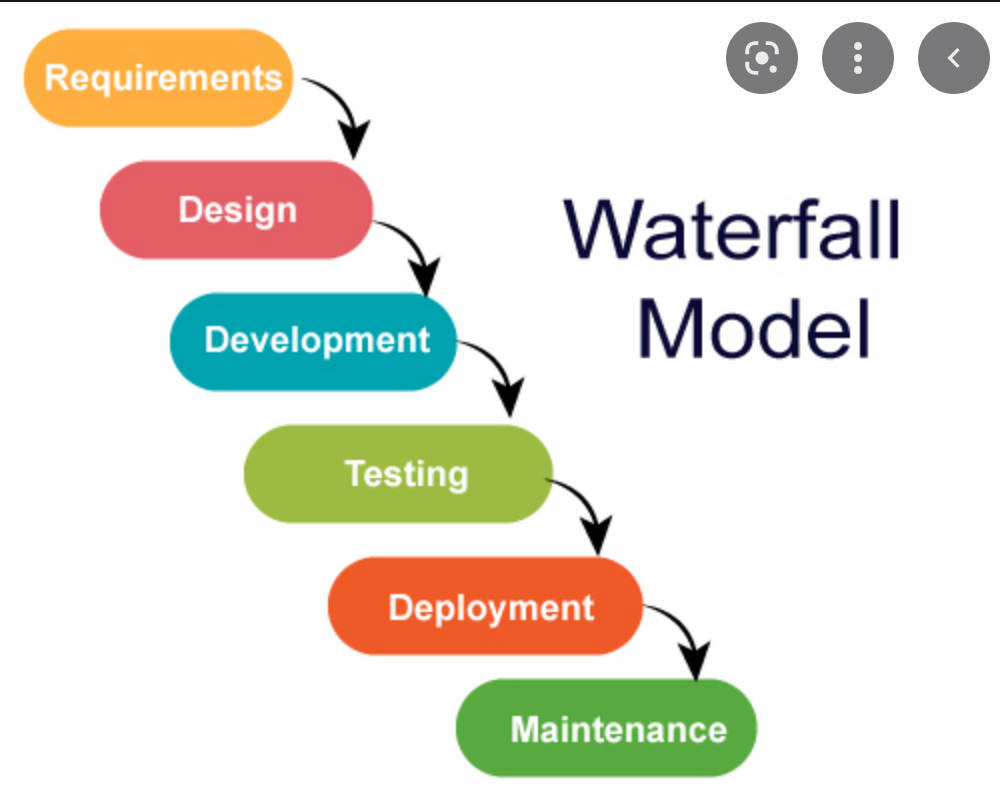
\includegraphics[width=0.8\linewidth]{img/image_2022-09-14-14-35-07.png}
	\caption{Waterfall method}
\end{figure}

In order to address this the V model was introduced which increases the amount of testing to reduce the possibility of having to rework everything
\begin{figure}[H]
	\centering
	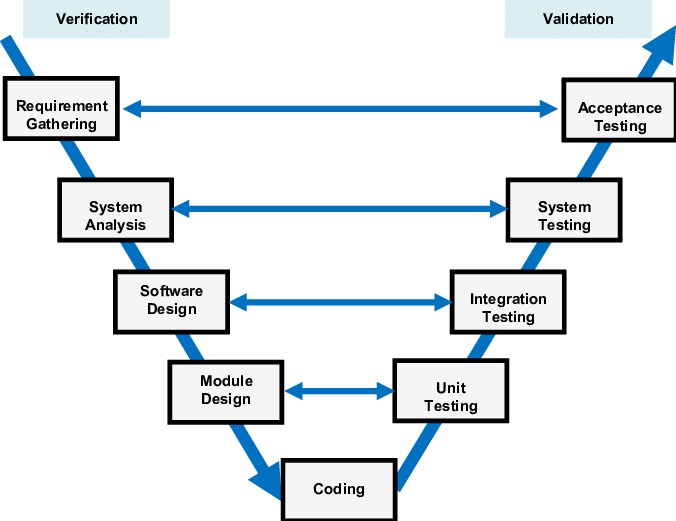
\includegraphics[width=0.8\linewidth]{img/image_2022-09-14-14-36-18.png}
	\caption{V model}
\end{figure}

Generally speaking the waterfall model isn't used much anymore due to the reality that software specifications change on a near daily basis.\marginnote{Recall: aUToronto Spring 2022 integration hell}


\subsubsection{Agile}

Agile is a project management approach which, in most general terms, seeks to respond to change and unpredictability using incremental, iterative work (sprints).
This allows for a balance between the need for predictability and the need for flexibility.
Some agile methods include:
\begin{itemize}
	\item Extreme programming: really really fast iteration (think days)
	\item Scrum: 2-4 week sprints with standups and backlogs; sticky notes for tasks, etc. Think kanban boards. Daily scrum meetings to unblock ASAP. Development lifecycle is therefore a series of sprints.
	\item On-site customer; frequent interaction with end users to figure out what exactly they need.
\end{itemize}


\subsection{I dropped this course}
\textbf{I decided to drop this course because the courseload was a little too much to handle between EngSci ECE, clubs, design teams, work, and trying to have a life.} 

\part{ESC301: Seminar}

\section{Preliminary}
\subsection{Seminar 1}


% \begin{thebibliography}{99}

% \end{thebibliography}


\end{document}






